\documentclass[color=black,11pt]{elegantpaper}
\usepackage{amsfonts} 
\usepackage{makecell} 
\usepackage{hyperref}
\usepackage{mathdots}
%\usepackage{makeindex}
%\makeindex
%\title{Euclidean space.} 
\title{\href{https://en.wikipedia.org/wiki/Euclidean_space}{Real Euclidean space}}
%\subtitle{Foundation of calculus}

\author{Sergey Nikitin}
%\institute{Elegant\LaTeX{} Program}
\date{January 20, 2025}
\version{1.0}
%\bioinfo{Bio}{Information}

%\extrainfo{Nihil est sine ratione. There is nothing without a reason.\\
%                         Gottfried Leibniz }

%\logo{spinning-calc.png}
%\cover{DSCF1445.JPG}

% modify the color in the middle of titlepage
\definecolor{customcolor}{RGB}{32,178,170}
\colorlet{coverlinecolor}{customcolor}

\begin{document}

\maketitle

%\frontmatter
%\tableofcontents

%\mainmatter

%%%%%%%%%%%%%%%%%introduction
\phantomsection
%\addcontentsline{toc}{chapter}{Introduction}
\section*{Introduction}
%\paragraph{Why another one? }


%\paragraph{ Framework}
 
This paper is about multidimensional real Euclidean spaces. First we build $n$-dimensional real linear space $\mathbb{R}^n$ out of $n$ copies of real line $\mathbb{R}.$ Each element of $\mathbb{R}^n$ is a string of $n$ real numbers $x=(x_1,\;x_2,\;\dots\;x_n).$ Note that $x \in \mathbb{R}^n$ is neither a point nor a vector. Instead, it is called a string of $n$ entries that are real numbers.  There is a reason for that. Terms such as point, vector come form geometry. However, we care less about geometry, mechanics, physics etc. We are talking only about real numbers that are names constructed out of a finite alphabet. $x\in \mathbb{R}^n$ means that $x$ consists of $n$ real numbers written next to each other. There is nothing else for it, period. We will rebuild all basic concepts you know from high school (straight line, plane, distance, angle, area, volume, projection) from scratch. \\
$\mathbb{R}^n$ endowed with operations of  addition, subtraction and multiplication by real numbers is a real linear space of $n$ dimensions. With those three operations one can not do much in $\mathbb{R}^n$ but only discuss linear affine subspaces of different dimensions. In particular, a straight line is a one dimensional affine linear subspace and a hyperplane is a $(n-1)$-dimensional affine linear subspace in $\mathbb{R}^n.$ In order to calculate all sorts of important stuff we need to update our trio with the following operation
$$
x\cdot y = x_1 \cdot y_1 + x_2 \cdot y_2 + \dots + x_n \cdot y_n.
$$
This is the dot product. $\mathbb{R}^n$ with the quartet of operations (addition/subtraction, multiplication by a number and the dot product) is called a Euclidean space. Due to the dot product we are able to calculate distances, angles, areas, volumes, projections etc. Note we do not need the cross product. Using the cross product to calculate areas, volumes or write an equation of a plane in $\mathbb{R}^3$ is one of those ridiculous antique traditions happily copy/pasted from a textbook to a textbook. The cross product plays important role in many areas of physics and mechanics. However, this cross product addiction looks a bit unhealthy. Moreover, by using formulas based on the cross product you lock yourself into a three dimensional cage (the cross product is defined only in $\mathbb{R}^3).$ Hopefully this text will cure you from the cross product mania. The cure is provided by $\ast$ operator and the wedge (exterior) product. Namely,
$$
\ast (a\wedge b)
$$  
is defined for $a,\;b\;\in \mathbb{R}^n$ and in $\mathbb{R}^3$ it coincides with the cross product.\\


Happy reading!!!\\
Sergey Nikitin 
 
%%%%%%%%%%%%%%%%%%%done with introduction




%\section{\href{https://en.wikipedia.org/wiki/Euclidean_space}{Real Euclidean space}}
\section{Two dimensional real linear space}
\label{sec:2space}
Consider a Cartesian product (see Definition ~\ref{def:Cartesian} in section ~\ref{sec:Metric}) 
$$
\mathbb{R} \times \mathbb{R} = \{(x_1,\;x_2);\;\;x_j \in \mathbb{R},\;j=1,\;2\}
$$  
It consists of strings of size two. We deliberately refrain from using widely accepted terminology like "points", "vectors"  instead we are talking about strings and their size is the number of their entries.  The widely accepted terminology pollutes our pure mathematical construction with some context that comes from geometry, mechanics, physics etc. However, at this point we do not care about applications yet.
\begin{definition}
\label{def:2space}
Given $x=(x_1,\;x_2)$ and $y=(y_1,\; y_2)$ we can define the following operations.
\begin{itemize}
\item[]Addition.
\begin{eqnarray*}
&& (x_1,\;x_2) \\
&+&\\
&& (y_1,\; y_2)\\
&&\overline{(x_1+y_1,x_2+y_2)}
\end{eqnarray*}
\item[]Subtraction.
\begin{eqnarray*}
&& (x_1,\;x_2) \\
&-&\\
&& (y_1,\; y_2)\\
&&\overline{(x_1-y_1,x_2-y_2)}
\end{eqnarray*}
\item[] Multiplication by a real number $\lambda \in \mathbb{R}.$
$$
\lambda \cdot x = (\lambda \cdot x_1,\; \lambda \cdot x_2)
$$
%\item[] \href{https://en.wikipedia.org/wiki/Dot_product}{Dot (scalar)  product.} 
%\begin{eqnarray*}
%&& (x_1,\;x_2) \\
%&\cdot&\\
%&& (y_1,\; y_2)\\
%x\cdot y&=&\overline{x_1\cdot y_1+x_2\cdot y_2}
%\end{eqnarray*}
\end{itemize}
The Cartesian product $\mathbb{R} \times \mathbb{R}$ together with those operations is called a two dimensional real linear space and denoted by $ \mathbb{R}^2.$
\end{definition}
Every $x \in \mathbb{R}^2, \;\;x=(x_1,\;x_2)$ can be written in one of the following form.\\
{\bf Column form:}
$$
x=x_1 \cdot \Big(\begin{array}{c}
                 1\\ 
                 0
            \end{array}\Big) + x_2 \cdot \Big(\begin{array}{c}
                                         0\\
                                         1
                                       \end{array}\Big)
$$
{\bf Row form:}
$$
x= x_1\cdot (1,\;0) + x_2 \cdot (0,\; 1)
$$
Let us introduce notations $e_1 =(1,\;0)$ and $e_2 = (0,\;1).$
The strings $e_1$ and $e_2 $ play special role in $\mathbb{R}^2,$
$$
x = x_1 \cdot e_1 + x_2 \cdot e_2
$$
for any $x\in \mathbb{R}^2.$ $\{e_1,\;e_2\}$ is called the canonical basis of $\mathbb{R}^2.$ \\
One can think about $\mathbb{R}^2$ as a digital model of a geometric plane (Fig. ~\ref{fig:plane}) like $\mathbb{R}$ being a digital model of a straight line. $\mathbb{R}$ is a one dimensional real linear space. Any zero string  (like $0,$ $(0,\;0)$ or $(0,\;\dots\;0)$) represents a $0$ dimensional linear space because addition, subtraction and multiplication by a real number for a zero strings yields again the same zero string.

\begin{figure}[htbp]
  \centering
  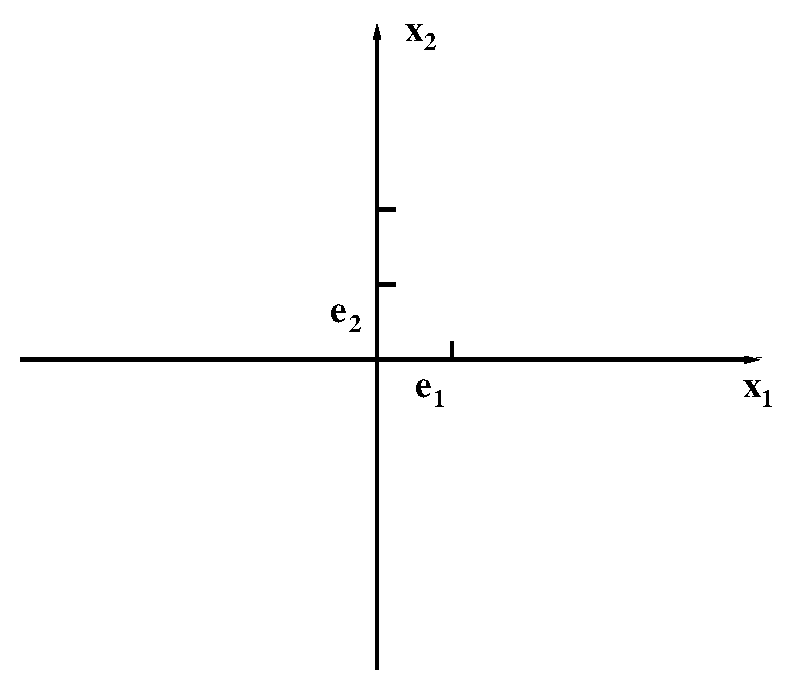
\includegraphics[width=0.6\textwidth]{xfig_stuff/plane.eps}
  \caption{Digitized plane is $\mathbb{R}^2$ with the canonical basis $\{e_1,\;e_2\}.$}
  \label{fig:plane}
\end{figure}

Given two strings $P,\;V\in \mathbb{R}^2$ we have
\begin{equation}
\label{eq:parametric_straight_line}
x = P+ t\cdot V,\;\;t\in \mathbb{R}
\end{equation} 
In geometrical jargon, this is a parametric equation of a straight line that contains the point with coordinates $P$ and goes in the direction of $V.$ The parameter $t$ can take any real value. In other words, $t$ labels points on the straight line. Type the lines depicted on Fig. ~\ref{fig:lineECandC} in \href{https://github.com/mathhobbit/EditCalculateAndChart/releases}{EditCalculateAndChart.}

\begin{figure}[htbp]
  \centering
  \includegraphics[width=0.6\textwidth]{image/lineECandC.png}
  \caption{Plotting $20$ points from the line in a parametric form}
  \label{fig:lineECandC}
\end{figure}
Highlight them and click the calculator button. You will see the points  (Fig. ~\ref{fig:lineECandCPlot}) from the following straight line.
$$
\Big(\begin{array}{c}
x_1\\
x_2
\end{array}\Big) = \Big(\begin{array}{c}
                              1\\
                              2
                   \end{array}\Big) + t \cdot \Big(\begin{array}{c}
                                      1\\
                                     -3
                                       \end{array}\Big) 
$$
\begin{figure}[htbp]
  \centering
  \includegraphics[width=0.6\textwidth]{image/lineECandCPlot.png}
  \caption{$20$ points from the line in a parametric form}
  \label{fig:lineECandCPlot}
\end{figure}
It follows from (~\ref{eq:parametric_straight_line}) that
$$
t\cdot V = x- P
$$
or in the entrywise form
\begin{eqnarray*}
t \cdot V_1 &=& x_1 - P_1\\
t \cdot V_2 &=& x_2 - P_2
\end{eqnarray*}
Since $t$ is the same in both the first and the second line we have
$$
\frac{x_1 - P_1}{V_1} = \frac{x_2 - P_2}{V_2}
$$
This is called a symmetric form of a straight line.\\
A straight line is also defined by
\begin{equation}
\label{eq:line}
a_1\cdot x_1 + a_2 \cdot x_2 = b
\end{equation}
where $a_1,\;a_2$ and  $b$ are real numbers.
\begin{center}
\begin{picture}(60,1)
\thicklines
\put(0,0){\line(1,0){60}}
\end{picture}
\end{center}
\begin{example}
Given points
\begin{eqnarray*}
A_1 &=& (1,\;-2)\\
A_2 &=& (3,\;4)
\end{eqnarray*}
find the equation (~\ref{eq:line}) of the straight line through $A_1,\;A_2.$\\
  Replacing $x_1,\;x_2$ in (~\ref{eq:line}) with the respective entries of $A_1$ and $A_2$ yields the following system of equations.
$$
\Big\{ \begin{array}{ccccc}
        a_1 &-&2\cdot a_2&=&b \\
        3\cdot a_1 &+&4\cdot a_2&=&b 
       \end{array}
$$
After multiplying the first equation by $2$ and adding the second we have
$$
\Big\{ \begin{array}{ccccc}
        5\cdot a_1 &&=&3\cdot b \\
        3\cdot a_1 &+&4\cdot a_2&=&b 
       \end{array}
$$
Hence, it follows from the first equation that 
$$
a_1 = \frac{3\cdot b}{5}
$$
and using it in the second equation we obtain
$$
a_2 = -\frac{b}{5}
$$
our formulas for $a_1,\;a_2$ transform (~\ref{eq:line}) into
$$
 \frac{3\cdot b}{5}\cdot x_1  -\frac{b}{5} \cdot x_2 = b
$$
Canceling $b$ (or putting $b=1)$ gives us the equation of the straight line through $A_1,\;A_2.$
$$
\frac{3}{5}\cdot x_1  -\frac{1}{5} \cdot x_2 = 1
$$ 
An equation for a straight line is defined up to multiplication by a number.  Therefore we can beautify our equation with multiplication by $5.$
$$
3\cdot x_1  - x_2 = 5
$$
Finally we can double check our answer by replacing $x_1,\;x_2$ with the respective entries for $A_1,\;A_2$ and making sure that the equation is valid.
\end{example}
\begin{center}
\begin{picture}(60,1)
\thicklines
\put(0,0){\line(1,0){60}}
\end{picture}
\end{center}

\section{$n$-dimensional real linear space}
\label{sec:nspace}
We already know that the straight line $\mathbb{R}$ is one dimensional real linear space. The plane $\mathbb{R}^2$ is two dimensional real linear space.

\begin{definition}
\label{def:nspace}
 $n$-dimensional real linear space is
$$
\mathbb{R}^n =\{(x_1,\; x_2,\; \dots \; x_n);\;x_j \in \mathbb{R}\;(j=1,\;2,\;\dots\;n)\}
$$
endowed with the following three operations.
\begin{itemize}
\item[]Addition.
\begin{eqnarray*}
&& (x_1,\;x_2,\;\dots\;x_n) \\
&+&\\
&& (y_1,\; y_2,\; \dots \; y_n)\\
&&\overline{(x_1+y_1,x_2+y_2, \; \dots \; x_n+y_n)}
\end{eqnarray*}
\item[]Subtraction.
\begin{eqnarray*}
&& (x_1,\;x_2,\;\dots\;x_n) \\
&-&\\
&& (y_1,\; y_2,\; \dots \; y_n)\\
&&\overline{(x_1-y_1,x_2-y_2, \; \dots \; x_n-y_n)}
\end{eqnarray*}
\item[] Multiplication by a real number $\lambda \in \mathbb{R}.$
$$
\lambda \cdot x = (\lambda \cdot x_1,\; \lambda \cdot x_2,\; \dots\; \lambda \cdot x_n)
$$
%\item[] \href{https://en.wikipedia.org/wiki/Dot_product}{Dot (scalar)  product.} 
%\begin{eqnarray*}
%&& (x_1,\;x_2) \\
%&\cdot&\\
%&& (y_1,\; y_2)\\
%x\cdot y&=&\overline{x_1\cdot y_1+x_2\cdot y_2}
%\end{eqnarray*}
\end{itemize}
\end{definition}
Every $x\in \mathbb{R}^n,\;\;x=(x_1,\;x_2,\;\dots\;x_n)$ can be written either in column or row form.\\
{\bf Column form:}\\
$$
x=x_1 \cdot \left(\begin{array}{c}
                 1\\
                 0\\ 
                 \vdots\\
                 0 
            \end{array}\right) + x_2 \cdot \left(\begin{array}{c}
                                         0\\
                                         1\\
                                       \vdots\\
                                         0
                                       \end{array}\right) + \dots + x_n \cdot \left(\begin{array}{c}
                                                                            0\\
                                                                         \vdots\\
                0\\ 
                                                                            1     
                                                                                  \end{array}\right)
$$
{\bf Row form:}\\
$$
x= x_1\cdot (1,\;0,\; \dots \; 0) + x_2 \cdot (0,\; 1,\; \dots \; 0) + \dots + x_n \cdot (0,\;0,\; \dots 1)
$$
The strings
\begin{eqnarray*}
e_1&=&(1,\;0,\; \dots\; 0)\\
e_2&=&(0,\;1,\; \dots\; 0)\\
&& \vdots\\
e_n&=&(0,\; \dots\; 0,\;1)\\
\end{eqnarray*}
define the canonical basis in $\mathbb{R}^n.$ For all $x\in \mathbb{R}^n$ we have
$$
x= x_1 \cdot e_1 + x_2 \cdot e_2 + \dots + x_n \cdot e_n
$$
Given $P,\;V\in \mathbb{R}^n$
\begin{equation}
\label{eq:ndline}
x= P+ t \cdot V\;\;\;t\in \mathbb{R}
\end{equation}
defines a straight line through $P$ in the direction of $V.$ It is a parametric equation of a straight line. $t\in \mathbb{R}$ is a parameter along the straight line. $t$ labels all points on the straight line.

\begin{center}
\begin{picture}(60,1)
\thicklines
\put(0,0){\line(1,0){60}}
\end{picture}
\end{center}
\begin{example}
Type and highlight the lines in \href{https://github.com/mathhobbit/EditCalculateAndChart/releases}{EditCalculateAndChart} (depicted on Fig. ~\ref{fig:3dline}).
\begin{figure}[htbp]
  \centering
  \includegraphics[width=0.6\textwidth]{image/3dline.png}
  \caption{Plotting the line in $\mathbb{R}^3$}
  \label{fig:3dline}
\end{figure}
By clicking with your mouse on the calculator icon (the last on the right ( Fig. ~\ref{fig:3dline})) you will plot the following line in $\mathbb{R}^3$ ( Fig. ~\ref{fig:3dlinePlot}).
\begin{figure}[htbp]
  \centering
  \includegraphics[width=0.6\textwidth]{image/3dlinePlot.png}
  \caption{The line in $\mathbb{R}^3$}
  \label{fig:3dlinePlot}
\end{figure}
$$
\Bigg(\begin{array}{c}
x_1\\
x_2\\
x_3
\end{array}\Bigg) = \left(\begin{array}{c}
                              1\\
                             -0.5\\
                              1.5 
                   \end{array}\right) + t \cdot \left(\begin{array}{c}
                                      2\\
                                      1\\
                                     -2
                                       \end{array}\right) 
$$
\end{example}
\begin{center}
\begin{picture}(60,1)
\thicklines
\put(0,0){\line(1,0){60}}
\end{picture}
\end{center}
It follows from (~\ref{eq:ndline}) that
\begin{eqnarray*}
tV_1 &=& x_1 - P_1\\
tV_2 &=& x_2 - P_2\\
&&\vdots\\
tV_n &=& x_n - P_n
\end{eqnarray*}
Since $t$ is the same in all the equations we obtain a symmetric form of a straight line,
$$
\frac{x_1 - P_1}{V_1} = \frac{x_2 - P_2}{V_2}=\dots = \frac{x_n - P_n}{V_n}
$$
A straight line  (~\ref{eq:ndline}) is a one dimensional affine linear subspace in $\mathbb{R}^n.$ In order to construct affine linear subspaces of dimensions higher than one we need the following new concept.
\begin{definition}
\label{def:linear_independence}
(\href{https://en.wikipedia.org/wiki/Linear_independence}{Linear independence})\\
The set of strings $\{V_1,\;V_2,\;\dots V_m\}$ from $\mathbb{R}^n$ is called linearly independent if, and only if,
$$
y_1 \cdot V_1 + y_2\cdot V_2+ \dots + y_m \cdot V_m =0
$$
only when $y_j = 0, j=1,\;2,\;\dots\;m.$ Otherwise it is linearly dependent. 
\end{definition}
Let $V_j \in \mathbb{R}^n ,\;\; j=1,\;2,\;\dots\;m$ be linearly independent. Let $P \in \mathbb{R}^n.$ Then the parametric equation
\begin{equation}
\label{eq:mspace}
x=P + t_1 \cdot V_1+ t_2 \cdot V_2 + \dots +t_m \cdot V_m,  \;\;\;(t_1,\;t_2,\;\dots\;t_m) \in \mathbb{R}^m 
\end{equation}
defines an $m$-dimensional \href{https://en.wikipedia.org/wiki/Affine_space#Affine_subspaces_and_parallelism}{affine linear subspace} in $\mathbb{R}^n.$ Every point of this \href{https://en.wikipedia.org/wiki/Affine_space#Affine_subspaces_and_parallelism}{affine subspace} is uniquely labeled by $m$ parameters $(t_1,\;t_2,\;\dots\;t_m) \in \mathbb{R}^m .$
\begin{center}
\begin{picture}(60,1)
\thicklines
\put(0,0){\line(1,0){60}}
\end{picture}
\end{center}
\begin{example}
Typing and highlighting the lines in \href{https://github.com/mathhobbit/EditCalculateAndChart/releases}{EditCalculateAndChart} (depicted on Fig. ~\ref{fig:3dplane}).
\begin{figure}[htbp]
  \centering
  \includegraphics[width=0.6\textwidth]{image/3dplane.png}
  \caption{Plotting the plane in $\mathbb{R}^3$}
  \label{fig:3dplane}
\end{figure}
Clicking the calculator icon with your mouse (the last icon in EditCalculateAndChart toolbar) will plot the plane in $\mathbb{R}^3$ (Fig. ~\ref{fig:3dplanePlot}). The plane is defined by the parametric equation
$$
\left(\begin{array}{c}
x_1\\
x_2\\
x_3
\end{array}\right) = \left(\begin{array}{c}
                              1\\
                              2\\
                             -1 
                   \end{array}\right) + t_1 \cdot \left(\begin{array}{c}
                                      1\\
                                      -1\\
                                       1 
                                       \end{array}\right) +t_2 \cdot \left(\begin{array}{c}
                                                                              -1\\
                                                                               3\\
                                                                               1
                                                                          \end{array}\right)
$$
\begin{figure}[htbp]
  \centering
  \includegraphics[width=0.6\textwidth]{image/3dplanePlot.png}
  \caption{The plane in $\mathbb{R}^3$}
  \label{fig:3dplanePlot}
\end{figure}
\end{example}
\begin{center}
\begin{picture}(60,1)
\thicklines
\put(0,0){\line(1,0){60}}
\end{picture}
\end{center}
It is well-known that a straight line is defined by two points. A plane in $\mathbb{R}^3$ is uniquely defined by three points that do not belong to a straight line. A similar statement remains true for a $m$-dimensional affine subspace in $\mathbb{R}^n.$ 
\begin{theorem}
A $m$-dimensional affine subspace in $\mathbb{R}^n$ is uniquely defined by $m+1$ points from $\mathbb{R}^n$ that do not belong to any $(m-1)$-dimensional affine subspace in $\mathbb{R}^n.$
\end{theorem}
\begin{proof}
Consider a  $m$-dimensional affine space defined by (~\ref{eq:mspace}). Let us denote it by $Sp(P;\;V_1,\;\dots\;V_m).$  The parameter $t=(t_1,\;t_2,\; \dots\; t_m)$ is from $\mathbb{R}^m.$ Taking 
$$
t=0,\;\mbox{ then } t=e_1,\;t=e_2,\;\dots\;t=e_m (\{e_1,\;\dots\;e_m\} \mbox{ is the canonical basis in } \mathbb{R}^m)
$$
yields $m+1$ points from $Sp(P;\;V_1,\;\dots\;V_m),$
$$
P,\; P+V_1,\;P+V_2,\;\dots\;P+V_m.
$$
These points do not belong to any  $(m-1)$-dimensional \href{https://en.wikipedia.org/wiki/Affine_space#Affine_subspaces_and_parallelism}{affine space} $Sp(Q;\;W_1,\;\dots\;W_{m-1})$ in $\mathbb{R}^n.$ Otherwise,
\begin{eqnarray}
\label{eq:points_in_subspace}
P&=& Q + \tau_{01} \cdot W_1+\tau_{02}\cdot W_2+\dots+\tau_{0\; m-1}\cdot W_{m-1} \nonumber \\
P+V_1&=& Q + \tau_{11} \cdot W_1+\tau_{12}\cdot W_2+\dots+\tau_{1\; m-1}\cdot W_{m-1} \nonumber\\
&&\vdots\\
P+V_m&=& Q + \tau_{m1} \cdot W_1+\tau_{m2}\cdot W_2+\dots+\tau_{m \;m-1}\cdot W_{m-1} \nonumber
\end{eqnarray}
and subtracting the first equation from all subsequent lines (~\ref{eq:points_in_subspace}) yields
\begin{eqnarray*}
V_1&=&  (\tau_{11}- \tau_{01}) \cdot W_1+(\tau_{12}-\tau_{02})\cdot W_2+\dots+(\tau_{1\; m-1}-\tau_{0\; m-1})\cdot W_{m-1} \\
&&\vdots\\
V_m&=&  (\tau_{m1} -\tau_{01}) \cdot W_1+(\tau_{m2} -\tau_{02})\cdot W_2+\dots+(\tau_{m \;m-1}-\tau_{0\; m-1})\cdot W_{m-1} 
\end{eqnarray*}
However, it contradicts to the assumption that $V_1,\;V_2,\;\dots \;V_m$ are linearly independent.\\
On the other hand, if the points
$$
P_0,\;P_1,\;\dots\;P_m
$$
do not belong to any $(m-1)$-dimensional affine subspace in $\mathbb{R}^n$ then 
$$
P_1 - P_0,\;P_2 -P_0,\;\dots\; P_m-P_0
$$
are linearly independent. Hence $P_0,\;P_1,\;\dots\;P_m$ uniquely define the $m$-dimensional affine linear subspace $Sp(P_0;\;P_1-P_0,\;\dots\;P_m-P_0)$ in $\mathbb{R}^n.$ 
\vspace{0.1cm}
Q.E.D.
\vspace{0.1cm}
\end{proof}
 A special place among affine linear subspaces in $\mathbb{R}^n$ is occupied by \href{https://en.wikipedia.org/wiki/Hyperplane}{hyperplanes} defined by
\begin{equation*}
\label{eq:hyper-plane}
a_1 \cdot x_1 + a_2 \cdot x_2+\dots + a_n\cdot x_n = b,
\end{equation*}
where $a_j\;\;(j=1,\;2,\;\dots \;n),\;b$ are real numbers. A hyperplane is a $(n-1)$-dimensional affine linear subspace of $\mathbb{R}^n.$

\begin{center}
\begin{picture}(60,1)
\thicklines
\put(0,0){\line(1,0){60}}
\end{picture}
\end{center}
\begin{example}
Given
\begin{eqnarray*}
A_1&=&(1,\;1,\;1,\;1)\\
A_2&=&(-1,\;-3,\;2,\;-2)\\
A_3&=&(1,\;9,\;4,\;4)\\
A_4&=&(-1,\;0,\;8,\;-8)\\
\end{eqnarray*}
find the hyperplane
\begin{equation}
\label{eq:4dhyperplane}
a_1\cdot x_1 + a_2 \cdot x_2 + a_3 \cdot x_3 +a_4 \cdot x_4 =b
\end{equation}
that contains $A_1, \;A_2,\;A_3,\; A_4.$ Substituting each of $A_1, \;A_2,\;A_3,\; A_4$ into (~\ref{eq:4dhyperplane}) leads us to the following system of equations.
\begin{equation}
\label{eq:4dsystem}
\left\{ \begin{array}{ccc}
        a_1 + a_2+\;\;\; a_3+\;\;\; a_4&=&b \\
        -a_1 -3\cdot a_2+2\cdot a_3- 2\cdot a_4&=&b \\
        a_1 +9\cdot a_2+4\cdot a_3+4 \cdot a_4&=&b \\
        -a_1 +0\cdot a_2+8\cdot a_3-8\cdot a_4&=&b 
       \end{array} \right.
\end{equation}
The procedure {\bf lslv} in \href{https://github.com/mathhobbit/EditCalculateAndChart/releases}{EditCalculateAndChart} can solve any linear system. Typing {\bf ?lslv}, highlighting and clicking the calculator button will give you the help instructions on how to use {\bf lslv}. \\
{\bf lslv(\{A\},\{r\})} will solve a linear system in \href{https://en.wikipedia.org/wiki/Matrix_(mathematics)}{the matrix form} $Ax=r.$ Instead of (~\ref{eq:4dsystem} ) we solve the following system
\begin{equation}
\label{eq:4dsystemuniform}
\left\{ \begin{array}{ccc}
        a_1 + a_2+\;\;\; a_3+\;\;\; a_4-b&=&0 \\
        -a_1 -3\cdot a_2+2\cdot a_3- 2\cdot a_4-b&=&0 \\
        a_1 +9\cdot a_2+4\cdot a_3+4 \cdot a_4-b&=&0 \\
        -a_1 +0\cdot a_2+8\cdot a_3-8\cdot a_4-b&=&0 
       \end{array} \right.
\end{equation}
for $(a_1,\; a_2,\; a_3,\; a_4,\; b).$ The next is the matrix form for (~\ref{eq:4dsystemuniform}).
$$
\left(\begin{array}{ccccc}
         1&1&1&1&-1\\
         -1&-3&2&-2&-1\\
         1&9&4&4&-1\\
         -1&0&8&-8&-1
      \end{array}\right)\left(\begin{array}{c}
                                  a_1\\
                                  a_2\\
                                  a_3\\
                                  a_4\\
                                  b
                              \end{array}\right)= \left(\begin{array}{c}
                                                           0\\
                                                           0\\
                                                           0\\
                                                           0
                                                         \end{array}\right) 
$$
The respective {\bf lslv} procedure for solving (~\ref{eq:4dsystemuniform}) is \\
{\bf lslv(\{1,\;1,\;1,\;1,\;-1;-1,\;-3,\;2,\;-2,\;-1;1,\;9,\;4,\;4,\;-1;-1,\;0,\;8,\;-8,\;-1\},\;\{0;0;0;0\}) } \\
Typing this line into  \href{https://github.com/mathhobbit/EditCalculateAndChart/releases}{EditCalculateAndChart}, highlighting and clicking the calculator button will solve this system (Fig. ~\ref{fig:lslv}).
\begin{figure}[htbp]
  \centering
  \includegraphics[width=0.6\textwidth]{image/lslv.png}
  \caption{Solving a linear system with {\bf lslv} }
  \label{fig:lslv}
\end{figure}
We have
$$
\left(\begin{array}{c}
           a_1\\
           a_2\\
           a_3\\
           a_4\\
           b
       \end{array}\right) = \left(\begin{array}{c}
                                \frac{7}{17}\\
                                -\frac{6}{17}\\
                                \frac{19}{34}\\
                                \frac{13}{34}\\
                                     1
                                   \end{array}\right)\cdot t,
$$
where $t$ is any nonzero value (the equation (~\ref{eq:4dhyperplane}) for hyperplane is defined up to a multiplication by a number). To beautify the answer we take $t=34.$  Then
$$
\left(\begin{array}{c}
           a_1\\
           a_2\\
           a_3\\
           a_4\\
           b
       \end{array}\right) = \left(\begin{array}{c}
                                14\\
                                -12\\
                                19\\
                                13\\
                                34 
                                   \end{array}\right)
$$
and the equation for the hyperplane is
$$
14\cdot x_1-12\cdot x_2 +19\cdot x_3 + 13 \cdot x_4 =34.
$$
You can double-check it by substituting into the equation the entries for $A_1, \;A_2,\;A_3,\; A_4$ and verifying that the equation holds.
\end{example}
\begin{center}
\begin{picture}(60,1)
\thicklines
\put(0,0){\line(1,0){60}}
\end{picture}
\end{center}
\section{Points and vectors are strings.}
A point $P$ from $\mathbb{R}^n$ is a string of size $n,$
$$
P=(P_1,\;P_2,\;\dots\; P_n)
$$ 
where $P_j\;\in\; \mathbb{R}\;\;(j=1,\;2,\; \dots \; n).$ Two points $P,\;Q\in \mathbb{R}^n$ define a vector $\overrightarrow{PQ},$
$$
\overrightarrow{PQ} = Q - P.
$$
 Any vector is defined by its head and tail. It is its head minus its tail. $Q$ is the head of $\overrightarrow{PQ}$ and $P$ is the tail of $\overrightarrow{PQ}.$\\
From the numerical point of view, there is no difference between vectors and points. They are both strings of a certain size. However, geometrically speaking they are different. One can think about  $\overrightarrow{PQ}$ as a mapping $S_{\overrightarrow{PQ}}$ of $\mathbb{R}^n$ into itself
$$
S_{\overrightarrow{PQ}}:\;\mathbb{R}^n \; \to\;\mathbb{R}^n
$$
 that shifts any $x\in\mathbb{R}^n$ into $x + \overrightarrow{PQ},$
$$   
S_{\overrightarrow{PQ}}(x) = x + \overrightarrow{PQ}.
$$
Any point $P$ can be considered as a vector which head is $P$ and tail is at the origin, $0.$ On the other hand, if you apply a vector $\overrightarrow{PQ}$ to the origin $0$ then the result is the point 
$$
S_{\overrightarrow{PQ}}(0)
$$
which is equal to the string $\overrightarrow{PQ}.$ Summarizing all this stuff  we can conclude that\\
\begin{center}
{\bf life is a mess.} 
\end{center}
The mess is created by mixing the geometrical concepts with something that just does not care about our human geometrical beliefs. Anyway, point and vector terminology could be sometimes convenient for our studies and we will occasionally use it in this manuscript. It is especially handy in $\mathbb{R}^2$ and $\mathbb{R}^3$ because we can engage our human geometrical intuition when solving  problems. In particular, all operations with strings (addition, subtraction, multiplication with a number (see definitions ~\ref{def:2space} and  ~\ref{def:nspace})) admit simple geometrical interpretations in $\mathbb{R}^2$ and $\mathbb{R}^3.$   The operations of addition and subtraction are depicted on Fig. ~\ref{fig:additiontriangle} and ~\ref{fig:vectorsubtraction}, respectively. For addition, instead of a triangle you can use the diagonal of a parallelogram (Fig. ~\ref{fig:additionparallelogram}). The sum $\vec{a}+\vec{b}+\vec{c}$  of three strings from $\mathbb{R}^3$ is the diagonal of a parallelepiped spanned by $\vec{a},\; \vec{b}\;$ and $\vec{c}.$

\begin{figure}[htbp]
  \centering
  \includegraphics[width=0.6\textwidth]{xfig_stuff/additiontrangle.eps}
  \caption{Vector addition in $\mathbb{R}^2$ and $\mathbb{R}^3.$ }
  \label{fig:additiontriangle}
\end{figure}
\begin{figure}[htbp]
  \centering
  \includegraphics[width=0.6\textwidth]{xfig_stuff/vectorsubtraction.eps}
  \caption{Vector subtraction in $\mathbb{R}^2$ and $\mathbb{R}^3.$ }
  \label{fig:vectorsubtraction}
\end{figure}
\begin{figure}[htbp]
  \centering
  \includegraphics[width=0.6\textwidth]{xfig_stuff/additionparallelogram.eps}
  \caption{Vector  addition in $\mathbb{R}^2$ and $\mathbb{R}^3.$ }
  \label{fig:additionparallelogram}
\end{figure}



\section{\href{https://en.wikipedia.org/wiki/Euclidean_space}{Euclidean space} is a linear space with the dot product}
\label{sec:Euclidean_space}
Linear real space $\mathbb{R}^n$ introduced in sections (~\ref{sec:2space}) and (~\ref{sec:nspace}) is equipped with three operations: addition, subtraction and multiplication by a numbers. It allows us to study affine linear subspaces in $\mathbb{R}^n.$ However, it does not give us any recipes on how to calculate distances, angles, areas, volumes. In order to close this gap we need the dot product.
\begin{definition}
(The dot product)\\ 
Given $x,\;y \in \mathbb{R}^n$ the dot product $x\cdot y$ is calculated  as follows.
\begin{eqnarray*}
&& (x_1,\;x_2,\;\dots\;x_n) \\
&\cdot&\\
&& (y_1,\; y_2,\; \dots \; y_n)\\
x\cdot y&=&\overline{x_1\cdot y_1+x_2\cdot y_2+ \; \dots \; +x_n\cdot y_n}
\end{eqnarray*}
\end{definition}
The dot product is a kind of a Pandora box that contains all you need in order to calculate all sorts of stuff that you know from your high school geometry classes. Moreover, everything, we are able to calculate with the dot product, is valid in $\mathbb{R}^n$  for any $n\in \mathbb{N}.$ It is cool, isn't it.\\
$\mathbb{R}^n$ endowed with the dot product is called a real Euclidean ($n$-dimensional) space and denoted again by $\mathbb{R}^n.$ The formal definition of a real Euclidean space follows.
\begin{definition}
\label{def:Euclidean_space}
(\href{https://en.wikipedia.org/wiki/Euclidean_space}{Euclidean space})\\

 $n$-dimensional real Euclidean space is
$$
\mathbb{R}^n =\{(x_1,\; x_2,\; \dots \; x_n);\;x_j \in \mathbb{R}\;(j=1,\;2,\;\dots\;n)\}
$$
endowed with the following four operations.
\begin{itemize}
\item[]Addition.
\begin{eqnarray*}
&& (x_1,\;x_2,\;\dots\;x_n) \\
&+&\\
&& (y_1,\; y_2,\; \dots \; y_n)\\
&&\overline{(x_1+y_1,x_2+y_2, \; \dots \; x_n+y_n)}
\end{eqnarray*}
\item[]Subtraction.
\begin{eqnarray*}
&& (x_1,\;x_2,\;\dots\;x_n) \\
&-&\\
&& (y_1,\; y_2,\; \dots \; y_n)\\
&&\overline{(x_1-y_1,x_2-y_2, \; \dots \; x_n-y_n)}
\end{eqnarray*}
\item[] Multiplication by a real number $\lambda \in \mathbb{R}.$
$$
\lambda \cdot x = (\lambda \cdot x_1,\; \lambda \cdot x_2,\; \dots\; \lambda \cdot x_n)
$$
\item[] \href{https://en.wikipedia.org/wiki/Dot_product}{Dot (scalar)  product.} 
\begin{eqnarray*}
&& (x_1,\;x_2,\; \dots \; x_n) \\
&\cdot&\\
&& (y_1,\; y_2,\; \dots \; y_n)\\
x\cdot y&=&\overline{x_1\cdot y_1+x_2\cdot y_2+\dots + x_n \cdot y_n}
\end{eqnarray*}
\end{itemize}
\end{definition}
\section{\href{https://en.wikipedia.org/wiki/Cauchy-Schwarz_inequality}{Cauchy-Schwarz inequality and distance}}
It follows from
$$
(u+t\cdot v)\cdot (u+t\cdot v)\ge 0 \;\;\;\forall\;t \in \mathbb{R}\;\;\mbox{ and } \forall\;\;u,\;v\in\mathbb{R}^n
$$
that
$$
(v \cdot v) \cdot t^2 + 2\cdot (v\cdot u) \cdot t + (u\cdot u) \ge 0 \;\;\forall\;t \in \mathbb{R}\;\;\mbox{ and } \forall\;\;u,\;v\in\mathbb{R}^n
$$
The \href{https://en.wikipedia.org/wiki/Quadratic_function}{quadratic polynomial} with respect to $t$ has at most one or none at all as far as real roots concerned.
Hence, its \href{https://en.wikipedia.org/wiki/Discriminant}{discriminant} is not positive,
$$
 (v\cdot u)^2-(v \cdot v) \cdot  (u\cdot u) \le 0
$$
and we obtain \href{https://en.wikipedia.org/wiki/Cauchy-Schwarz_inequality}{Cauchy-Schwarz inequality}
$$
|v\cdot u | \le \sqrt{(v \cdot v)}\cdot \sqrt{(u\cdot u)}.
$$
Let us introduce notation $|u|=\sqrt{u\cdot u}.$ Then \href{https://en.wikipedia.org/wiki/Cauchy-Schwarz_inequality}{Cauchy-Schwarz inequality} takes this form
$$
|v\cdot u | \le |u| \cdot |v|.
$$
$|u|$ is called  a magnitude (or absolute value) of $u\in \mathbb{R}^n.$ 
$$
|v\cdot u | = |u| \cdot |v|.
$$
if, and only if,  $u+t\cdot v = 0$ for some $t.$ In this case we are saying that $u$ and $v$ are \href{https://en.wikipedia.org/wiki/Collinearity}{collinear} (or \href{https://en.wikipedia.org/wiki/Parallel_(geometry)}{parallel}).
\begin{definition}
(Distance)\\
The distance between $A\in \mathbb{R}^n$ and  $B\in \mathbb{R}^n$ is defined by
$$
|B-A|=\sqrt{(B-A)\cdot (B-A)}.
$$
\end{definition}
Real Euclidean space $\mathbb{R}^n$ with the distance function $|x-y|$ is a metric space (see section ~\ref{sec:Metric}). It is easy to see that $|x-y|$ has reflexivity and symmetricity properties. The triangle property follows from \href{https://en.wikipedia.org/wiki/Cauchy-Schwarz_inequality}{Cauchy-Schwarz inequality}.   Indeed,
\begin{eqnarray*}
|x-z| &=& |x-y + y-z|=\sqrt{(x-y + y-z )\cdot (x-y + y-z) }=\\
&&\sqrt{(x-y)\cdot (x-y) +2\cdot (x-y)\cdot ( y-z) +( y-z)\cdot ( y-z) } =\\
&&\sqrt{|x-y|^2 +2\cdot (x-y)\cdot ( y-z) +| y-z|^2}\le\\
&& \sqrt{|x-y|^2+ 2\cdot |x-y|\cdot | y-z|+| y-z|^2 }=|x-y| + | y-z|
\end{eqnarray*}

\begin{center}
\begin{picture}(60,1)
\thicklines
\put(0,0){\line(1,0){60}}
\end{picture}
\end{center}
\begin{example}
Determine whether the three points 
\begin{eqnarray*}
A_1 &=&(2,\;0,\;3,1)\\
A_2 &=&(1,\;1,\;1,\;1)\\
A_3 &=&(3,\; -1,\;5,\;1)
\end{eqnarray*}
are \href{https://en.wikipedia.org/wiki/Collinearity}{collinear} (all sitting on a straight line). There are several ways to solve this problem.\\
  The first is based on \href{https://en.wikipedia.org/wiki/Cauchy-Schwarz_inequality}{Cauchy-Schwarz inequality}. Calculating
\begin{eqnarray*}
A_1 - A_2 &=& (1,\;-1,\;2,\;0)\\
A_3 - A_2 &=& (2,\;-2,\;4,\;0) 
\end{eqnarray*}
and
\begin{eqnarray*}
(A_1 - A_2)\cdot (A_3 - A_2) &=& 12\\
|A_1 - A_2| &=& \sqrt{6}\\
|A_3 - A_2| &=& \sqrt{24} 
\end{eqnarray*}
yields
\begin{eqnarray*}
(A_1 - A_2)\cdot (A_3 - A_2) &=& |A_1 - A_2| \cdot |A_3 - A_2|\\
12 &=& \sqrt{6} \cdot \sqrt{24}
\end{eqnarray*}
By \href{https://en.wikipedia.org/wiki/Cauchy-Schwarz_inequality}{Cauchy-Schwarz inequality} it is possible if, and only if, $A_1 - A_2$ and $A_3 - A_2$ are collinear and so are the points in question. \\
The second method is to calculate distances.
\begin{eqnarray*}
|A_1 - A_3| &=& \sqrt{6}\\
|A_1 - A_2| &=& \sqrt{6}\\
|A_3 - A_2| &=& \sqrt{24}=2\cdot \sqrt{6} 
\end{eqnarray*}
Since
$$
|A_3 - A_2| = |A_1 - A_2| + |A_1 - A_3|
$$
the points $A_1,\;A_2,\;A_3$ are collinear (Fig. ~\ref{fig:collinearpoints}).
\begin{figure}[htbp]
  \centering
  \includegraphics[width=0.6\textwidth]{xfig_stuff/collinearpoints.eps}
  \caption{$A_1,\;A_2,\;A_3$ are collinear points }
  \label{fig:collinearpoints}
\end{figure}

\end{example}
\begin{center}
\begin{picture}(60,1)
\thicklines
\put(0,0){\line(1,0){60}}
\end{picture}
\end{center}
\section{Angle and area}
\label{angle_area}
An angle between any two strings $a,\;b\; \in \mathbb{R}^n \;(a\not=0,\;\;b\not= 0)$ is calculated with the help of the dot product. 
\begin{definition}
(Angle)\\
Cosine $\cos(\hat{ab})$ of the angle $\hat{ab}$ between any $a,\;b\; \in \mathbb{R}^n \;(a\not=0,\;\;b\not= 0)$ is equal to
$$
\cos(\hat{ab}) = \frac{a\cdot b}{|a|\cdot |b|}
$$
and
$$
\hat{ab} = \arccos(\frac{a\cdot b}{|a|\cdot |b|})
$$
\end{definition}

\begin{center}
\begin{picture}(60,1)
\thicklines
\put(0,0){\line(1,0){60}}
\end{picture}
\end{center}
\begin{example}
Calculate the angle $\hat{ab}$ between
\begin{eqnarray*}
a&=&(1,-1,1,3,-4,6)\\
b&=&(3,8,11,9,4,-6)
\end{eqnarray*}
We use \href{https://github.com/mathhobbit/EditCalculateAndChart/releases}{EditCalculateAndChart} to solve this problem (Fig. ~\ref{fig:angle}).
\begin{figure}[htbp]
  \centering
  \includegraphics[width=0.6\textwidth]{image/angle.png}
  \caption{Calculating angle $\hat{ab}.$ }
  \label{fig:angle}
\end{figure}
\end{example}
\begin{center}
\begin{picture}(60,1)
\thicklines
\put(0,0){\line(1,0){60}}
\end{picture}
\end{center}
The area of a parallelogram spanned by two strings $a\in \mathbb{R}^n$ and $b\in \mathbb{R}^n$ (Fig. ~\ref{fig:parallelogram})  also is calculated with the help of the dot product.
\begin{figure}[htbp]
  \centering
  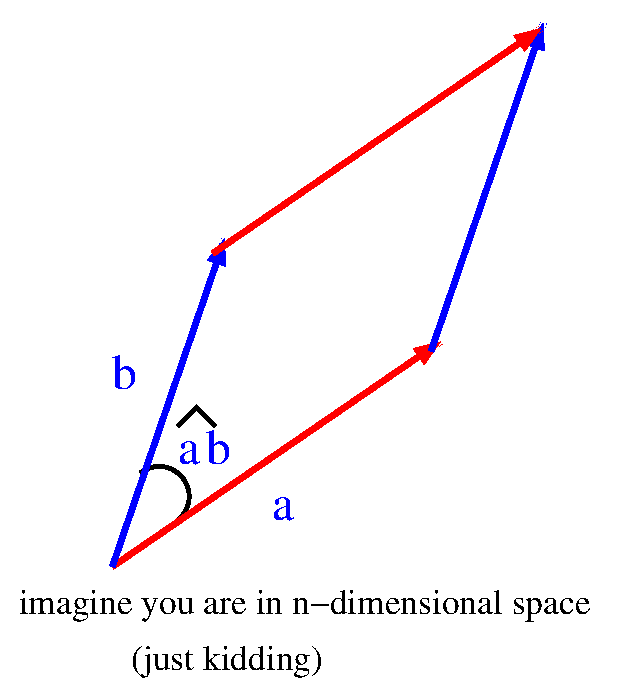
\includegraphics[width=0.6\textwidth]{xfig_stuff/parallelogram.eps}
  \caption{Parallelogram spanned by $a\in \mathbb{R}^n$ and $b\in \mathbb{R}^n.$ }
  \label{fig:parallelogram}
\end{figure}
\begin{definition}
(Area)\\
Let $a,\;b\in \mathbb{R}^n.$ Then the area of parallelogram spanned by $a$ and $b$ is equal to
\begin{equation}
\label{eq:determinant_area}
\sqrt{\det\left( \begin{array}{cc}
             a\cdot a& a\cdot b\\
             b\cdot a& b\cdot b
           \end{array} \right)},
\end{equation}
where \href{https://en.wikipedia.org/wiki/Determinant}{the determinant} of a $2 \times 2$-matrix is calculated as follows.
$$
\det \left( \begin{array}{cc}
a_{1\; 1}& a_{1\; 2}\\
a_{2\; 1} & a_{2\; 2} 
\end{array} \right) = a_{1\; 1} \cdot a_{2\; 2} - a_{1\; 2} \cdot a_{2\; 1}
$$
\end{definition}
In high school you probably learned another good formula for the area of parallelogram spanned by $a,\; b \in \mathbb{R}^n,$
\begin{equation}
\label{eq:geometric_area}
\mbox{ area }=|a|\cdot |b| \sin(\hat{ab}).
\end{equation}
Let us show that (~\ref{eq:determinant_area}) and (~\ref{eq:geometric_area}) are the same.\\
Since
$$
\mbox{ area }=|a|\cdot |b| \sin(\hat{ab}) = |a|\cdot |b|\sqrt{1- \cos^2(\hat{ab})} =\sqrt{|a|^2 \cdot |b|^2 - (|a|\cdot |b|  \cos(\hat{ab}))^2}
$$
and taking into account that
$$
|a|^2 = a\cdot a,\;\;|b|^2 = b\cdot b,\;\;|a|\cdot |b|  \cos(\hat{ab}) = a\cdot b
$$
we obtain
$$
\sqrt{|a|^2 \cdot |b|^2 - (|a|\cdot |b|  \cos(\hat{ab}))^2} = \sqrt{\det\left( \begin{array}{cc}
             a\cdot a& a\cdot b\\
             b\cdot a& b\cdot b  
           \end{array} \right)}
$$
that yields
$$
\mbox{ area }=|a|\cdot |b| \sin(\hat{ab})=\sqrt{\det\left( \begin{array}{cc}
             a\cdot a& a\cdot b\\
             b\cdot a& b\cdot b
           \end{array} \right)} 
$$

In $\mathbb{R}^2$ the formula for area takes especially simple form.\\
Suppose that $a,\;b\in \mathbb{R}^2,$
\begin{eqnarray*}
a &=& (a_1,\;a_2)\\
b &=& (b_1,\;b_2)
\end{eqnarray*}
Then
$$
\left( \begin{array}{cc}
             a\cdot a& a\cdot b\\
             b\cdot a& b\cdot b
           \end{array} \right) = \left( \begin{array}{cc}
             a_1& a_2\\
             b_1&  b_2
           \end{array} \right)\cdot \left( \begin{array}{cc}
             a_1&  b_1\\
             a_2&  b_2
           \end{array} \right)
$$
It is well known that the determinant of the product is equal to the product of the determinants. The reader also can easily see that
$$
\det \left( \begin{array}{cc}
             a_1& a_2\\
             b_1&  b_2
           \end{array} \right) = \det \left( \begin{array}{cc}
             a_1&  b_1\\
             a_2&  b_2
           \end{array} \right)
$$
Thus
$$
\mbox{ area } = \sqrt{\det\left( \begin{array}{cc}
             a\cdot a& a\cdot b\\
             b\cdot a& b\cdot b
           \end{array} \right)}=|\det \left( \begin{array}{cc}
             a_1& a_2\\
             b_1&  b_2
           \end{array} \right)|.
$$
This formula for the area works \textcolor{red}{ONLY IN $\mathbb{R}^2$}.
$$
\mbox{ area } = |\det \left( \begin{array}{cc}
             a_1& a_2\\
             b_1&  b_2
           \end{array} \right)|.
$$
\section{\href{https://en.wikipedia.org/wiki/Volume}{Volume}}
Calculation of volumes in $\mathbb{R}^n$ is sort of similar to calculation of areas. We need only the dot product in order to find the volume of the parallelepiped spanned by $a,\;b \in \mathbb{R}^n$ and $c\in \mathbb{R}^n.$
\begin{definition}
(Volume)\\
Let $a,\;b,\; c\in \mathbb{R}^n.$ Then the volume of parallelepiped spanned by $a,\;b$ and $c$ is equal to
\begin{equation*}
%\label{eq:determinant_volume}
\sqrt{\det\left( \begin{array}{ccc}
             a\cdot a& a\cdot b & a \cdot c\\
             b\cdot a& b\cdot b & b \cdot c\\
             c\cdot a& c\cdot b & c \cdot c
           \end{array} \right)},
\end{equation*}
where \href{https://en.wikipedia.org/wiki/Determinant}{the determinant} of a $3 \times 3$-matrix is calculated as follows.
\begin{eqnarray*}
\det \left( \begin{array}{ccc}
a_{1\; 1}& a_{1\; 2} & a_{1\; 3}\\
a_{2\; 1} & a_{2\; 2}& a_{2\; 3}\\ 
a_{3\; 1} & a_{3\; 2}& a_{3\; 3} 
\end{array} \right) &=& a_{1\; 1} \cdot a_{2\; 2}\cdot a_{3\; 3} + a_{2\; 1} \cdot a_{3\; 2} \cdot  a_{1\; 3} + a_{1\; 2} \cdot a_{2\; 3} \cdot a_{3\; 1} \\
&&-a_{1\; 3} \cdot  a_{2\; 2} \cdot a_{3\; 1}  -  a_{1\; 2} \cdot a_{2\; 1} \cdot a_{3\; 3} - a_{2\; 3}\cdot a_{3\; 2} \cdot a_{1\; 1}
\end{eqnarray*}
\end{definition}
The formula for volume takes an especially simple form in $\mathbb{R}^3.$  Indeed, if $a,\;b,\;c  \mathbb{R}^3,$ then
\begin{eqnarray*}
a&=&(a_1,\; a_2,\; a_3)\\
b&=&(b_1,\; b_2,\; b_3)\\
c&=&(c_1,\; c_2,\; c_3)
\end{eqnarray*}
and
$$
\left( \begin{array}{ccc}
             a\cdot a& a\cdot b & a \cdot c\\
             b\cdot a& b\cdot b & b \cdot c\\
             c\cdot a& c\cdot b & c \cdot c
           \end{array} \right)= \left( \begin{array}{ccc}
                                        a_1 & a_2 & a_3\\ 
                                        b_1 & b_2 & b_3\\ 
                                        c_1 & c_2 & c_3 
                                        \end{array} \right)\cdot \left( \begin{array}{ccc}
                                                                         a_1 & b_1 & c_1\\
                                                                         a_2 & b_2 & c_2\\
                                                                         a_3 & b_3 & c_3
                                                                         \end{array} \right)
$$
The \href{https://en.wikipedia.org/wiki/Determinant}{determinant} of the product is the product of  the determinants. It follows from
$$
\det \left( \begin{array}{ccc}
                                        a_1 & a_2 & a_3\\
                                        b_1 & b_2 & b_3\\
                                        c_1 & c_2 & c_3
                                        \end{array} \right)= \det \left( \begin{array}{ccc}
                                                                         a_1 & b_1 & c_1\\
                                                                         a_2 & b_2 & c_2\\
                                                                         a_3 & b_3 & c_3  
                                                                         \end{array} \right)
$$
that
$$
\mbox{ volume } = \sqrt{\det \left( \begin{array}{ccc}
             a\cdot a& a\cdot b & a \cdot c\\
             b\cdot a& b\cdot b & b \cdot c\\
             c\cdot a& c\cdot b & c \cdot c
           \end{array} \right)  } = |\det \left( \begin{array}{ccc}
                                        a_1 & a_2 & a_3\\
                                        b_1 & b_2 & b_3\\
                                        c_1 & c_2 & c_3
                                        \end{array} \right) |.
$$
This formula for the volume works \textcolor{red}{ONLY IN $\mathbb{R}^3$}.
$$
\mbox{ volume } = |\det \left( \begin{array}{ccc}
                                        a_1 & a_2 & a_3\\
                                        b_1 & b_2 & b_3\\
                                        c_1 & c_2 & c_3
                                        \end{array} \right) |.
$$


\section{The distance between a point and a linear affine subspace in $\mathbb{R}^n$}
Consider a point $Q \in \mathbb{R}^n$ and a straight line in a parametric form
\begin{equation}
\label{eq:strline}
x = P + t\cdot V,\;\;t \in \mathbb{R}
\end{equation}
where $P,\;V \; \in \mathbb{R}^n.$ The idea of calculating the distance \textcolor{red}{$d$} from $Q$ to the straight line (~\ref{eq:strline}) is depicted on Fig. ~\ref{fig:distancePointLine}). The distance \textcolor{red}{$d$} is the area of the parallelogram divided by $|V|.$ We know how to calculate the area of a parallelogram in $\mathbb{R}^n$ ( see section ~\ref{angle_area}).
\begin{figure}[htbp]
  \centering
  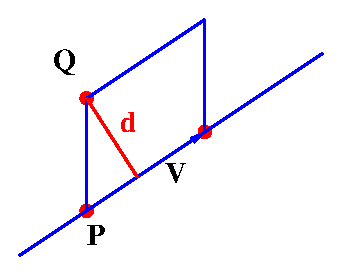
\includegraphics[width=0.6\textwidth]{xfig_stuff/distancePointLine.eps}
  \caption{Area of parallelogram is $|V|\cdot$\textcolor{red}{$ d$}.}
  \label{fig:distancePointLine}
\end{figure}

The distance between $Q$ and the straight line (~\ref{eq:strline}) is given by the formula
$$
\frac{\sqrt{\det \left(\begin{array}{cc}
                           (Q-P) \cdot (Q-P) & (Q-P) \cdot V\\
                            V \cdot (Q-P)  & V\cdot V 
                       \end{array}  \right)}}{|V|}
$$
The same idea works for calculating the distance between  $Q \in \mathbb{R}^n$ and a $m$-dimensional affine linear subspace in $\mathbb{R}^n$ spanned by $V_1,\;V_2,\; \dots V_m.$ However, we need to introduce a new concept, $m$-dimensional volume or $m$-volume.
\begin{definition}
\label{def:mvolume}
($m$-volume)\\
Given linearly independent  $V_1,\;V_2,\; \dots  V_m$ their volume is denoted by $Vol (V_1,\;V_2,\;\dots \;V_m)$ and calculated as follows.
\begin{equation}
\label{mvolume}
Vol (V_1,\;V_2,\;\dots \;V_m) = \sqrt{\det \left(\begin{array}{cccc}
                                                    V_1\cdot V_1 & V_1\cdot V_2& \dots & V_1 \cdot V_m\\
                                                    V_2\cdot V_1 & V_2\cdot V_2& \dots & V_2 \cdot V_m\\
                                                        \vdots &\vdots &\dots &\vdots \\
                                                    V_m\cdot V_1 & V_m\cdot V_2& \dots & V_m \cdot V_m
                                                   \end{array}  \right) }
\end{equation}
\end{definition}
In order to calculate \href{https://en.wikipedia.org/wiki/Determinant}{the determinant} of $m\times m$-matrix (with $m$ rows and $m$ columns) 
$$
\det \left(\begin{array}{cccc}
                 a_{1\; 1} & a_{1\; 2} & \dots & a_{1\; m}\\
                 a_{2\; 1} & a_{2\; 2} & \dots & a_{2\; m}\\
                   \vdots & \vdots & \dots &\vdots \\
                 a_{m\; 1} & a_{m\; 2} & \dots & a_{m\; m}
           \end{array}  \right)
$$
we use \href{https://en.wikipedia.org/wiki/Laplace_expansion}{Laplace rule}. We choose either a row or a column of the matrix. Assume that we have chosen  $j$th row
$$
                 a_{j\; 1} \;\; a_{j\; 2} \;\; \dots \;\; a_{j\; m}
$$
Then we pick elements one by one from the $j$the row and calculate the determinant. 
$$
\det \left(\begin{array}{cccc}
                 a_{1\; 1} & a_{1\; 2} & \dots & a_{1\; m}\\
                 a_{2\; 1} & a_{2\; 2} & \dots & a_{2\; m}\\
                   \vdots & \vdots & \dots &\vdots \\
                 a_{m\; 1} & a_{m\; 2} & \dots & a_{m\; m}
           \end{array}  \right)= \sum_{k=1}^m (-1)^{j+k} a_{j\; k} \cdot M_{j\; k},
$$

where $M_{j\; k}$ denotes the $jk$th minor of the matrix. The minor  $M_{j\; k}$ is the determinant of the matrix obtained by crossing out $j$th row and $k$th column from 
$$
\left(\begin{array}{cccc}
                 a_{1\; 1} & a_{1\; 2} & \dots & a_{1\; m}\\
                 a_{2\; 1} & a_{2\; 2} & \dots & a_{2\; m}\\
                   \vdots & \vdots & \dots &\vdots \\
                 a_{m\; 1} & a_{m\; 2} & \dots & a_{m\; m}  
           \end{array}  \right).
$$
If we picked $j$th column instead of $j$th row then Laplace rule would yield
$$
\det \left(\begin{array}{cccc}
                 a_{1\; 1} & a_{1\; 2} & \dots & a_{1\; m}\\
                 a_{2\; 1} & a_{2\; 2} & \dots & a_{2\; m}\\
                   \vdots & \vdots & \dots &\vdots \\
                 a_{m\; 1} & a_{m\; 2} & \dots & a_{m\; m}
           \end{array}  \right)= \sum_{k=1}^m (-1)^{k+j} a_{k\; j} \cdot M_{k\; j},
$$
Given $P\in\mathbb{R}^n$ and linearly independent $V_1,\;V_2,\; \dots \; V_m$ from $\mathbb{R}^n$ the distance between $Q\in \mathbb{R}^n$ and a linear affine space
$$
x= P + t_1 \cdot V_1+t_2 \cdot V_2 + \dots + t_m V_m,\;\;\; t_j \in \mathbb{R}\;(j=1,\;2,\; \dots \; m)
$$
 is calculated with the formula
$$
\frac{Vol(Q-P,\;V_1,\;V_2,\;\dots \; V_m)}{Vol(V_1,\;V_2,\;\dots \; V_m)}
$$ 
where $Vol$ is defined in (~\ref{mvolume}).
\section{Orthogonal projection}
Orthogonal projection of $u\in \mathbb{R}^n$ onto $v\in \mathbb{R}^n$ is depicted on Fig. ~\ref{fig:orthogonalProjection}.
\begin{figure}[htbp]
  \centering
  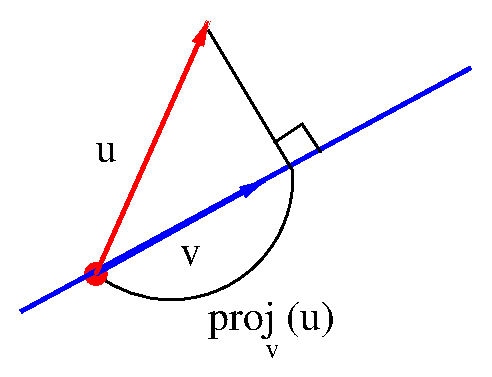
\includegraphics[width=0.6\textwidth]{xfig_stuff/orthogonalProjection.eps}
  \caption{Orthogonal projection $proj_v(u)$ of $u$ onto $v$.}
  \label{fig:orthogonalProjection}
\end{figure}
\begin{definition}
\href{https://mathworld.wolfram.com/Orthogonal.html}{(Orthogonal)}\\
Two strings $a,\;b\in \mathbb{R}^n$ are called \href{https://mathworld.wolfram.com/Orthogonal.html}{orthogonal} if  the angle $\hat{ab}=\frac{\pi}{2}$ or
$$
a \cdot b = 0.
$$
\end{definition}
If $proj_v(u)$ is the orthogonal projection of $u$ onto $v$ then $u- proj_v(u)$ is orthogonal to $v,$
\begin{equation}
\label{eq:projection}
(u- proj_v(u))\cdot v = 0.
\end{equation}
As we can see (Fig. ~\ref{fig:orthogonalProjection}) $proj_v(u)$ is the multiple of $v,$
$$
proj_v(u) = \lambda \cdot v
$$
and it follows from (~\ref{eq:projection}) that
$$
u\cdot v = \lambda \cdot v\cdot v
$$ 
Hence,
$$
\lambda = \frac{u\cdot v}{v\cdot v}
$$
and 
$$
proj_v(u) = \frac{u\cdot v}{v\cdot v} \cdot v
$$
or, taking into account that $v\cdot v=|v|^2,$
$$
proj_v(u) = \frac{u\cdot v}{|v|^2} \cdot v.
$$
Note that 
$$
e_v=\frac{v}{|v|}
$$
is \href{https://en.wikipedia.org/wiki/Unit_vector}{the unit vector} in the direction of $v.$
Thus,
$$
proj_v(u) = \frac{u\cdot v}{|v|} \cdot e_v
$$
The coefficient
$$
\frac{u\cdot v}{|v|}
$$
is called \href{https://en.wikipedia.org/wiki/Scalar_projection}{the scalar projection} of $u$ onto $v.$\\

Consider a linear subspace from $\mathbb{R}^n$ spanned by linearly independent $V_1,\;V_2,\; \dots \; V_m$ from $\mathbb{R}^n,$ 
$$
Spann(V_1,V_2,\dots,V_m)=\{ t_1 \cdot V_1+t_2 \cdot V_2 + \dots + t_m V_m;\;\;\; t_j \in \mathbb{R}\;(j=1,\;2,\; \dots \; m)\}.
$$
If $proj(u;V_1,V_2,\dots,V_m)$ is the orthogonal projection of $u$ onto $Spann(V_1,V_2,\dots,V_m)$ then $u- proj_v(u;V_1,V_2,\dots,V_m)$ is orthogonal to $Spann(V_1,V_2,\dots,V_m),$
\begin{equation}
\label{eq:projection_onto_spann}
(u- proj_v(u;V_1,V_2,\dots,V_m))\cdot V_j = 0\;\;\mbox{ for }\;\;j=1,\;2,\; \dots \; m
\end{equation}
Taking into account that
\begin{equation}
\label{eq:projection_onto_spann_1}
proj_v(u;V_1,V_2,\dots,V_m) = \lambda_1 \cdot V_1 + \lambda_2 \cdot V_2 +\dots + \lambda_m \cdot V_m
\end{equation}
we derive from (~\ref{eq:projection_onto_spann}) the following linear system for $(\lambda_1, \;\lambda_2,\;\dots, \;\lambda_m).$
\begin{equation}
\label{eq:Gramm_system}
\left(\begin{array}{cccc}
             V_1 \cdot V_1 & V_1 \cdot V_2 & \dots & V_1 \cdot V_m\\
             V_2 \cdot V_1 & V_2 \cdot V_2 & \dots & V_2 \cdot V_m\\
             \vdots & \vdots & \dots &\vdots \\
             V_m \cdot V_1 & V_m \cdot V_2 & \dots & V_m \cdot V_m
      \end{array}  \right)\left(\begin{array}{c} 
                                \lambda_1\\
                                \lambda_2\\
                                  \vdots \\
                                \lambda_m
                                \end{array}
                          \right)
                          = \left(\begin{array}{c}
                               V_1 \cdot u\\
                               V_2 \cdot u\\
                                  \vdots \\
                               V_m \cdot u
                                \end{array}
                           \right)
\end{equation}
The matrix of this linear system of equations is named after Danish mathematician, \href{https://en.wikipedia.org/wiki/J%C3%B8rgen_Pedersen_Gram}{J.P. Gram.} It is called \href{https://en.wikipedia.org/wiki/Gram_matrix}{the Gramm matrix} (of $V_1,\;V_2,\; \dots \; V_m)$ and is denoted by
$$
 G(V_1,\;V_2,\; \dots \; V_m) = \left(\begin{array}{cccc}
             V_1 \cdot V_1 & V_1 \cdot V_2 & \dots & V_1 \cdot V_m\\
             V_2 \cdot V_1 & V_2 \cdot V_2 & \dots & V_2 \cdot V_m\\
             \vdots & \vdots & \dots &\vdots \\
             V_m \cdot V_1 & V_m \cdot V_2 & \dots & V_m \cdot V_m
      \end{array}  \right)
$$
The determinant $det( G(V_1,\;V_2,\; \dots \; V_m))$ is called the Grammian (of $V_1,\;V_2,\; \dots \; V_m).$ Since $V_1,\;V_2,\; \dots \; V_m$ are linearly independent the Grammian of  $V_1,\;V_2,\; \dots \; V_m$ is not zero and the system (~\ref{eq:Gramm_system}) admits the unique solution,
$$
   \lambda = (G(V_1,\;V_2,\; \dots \; V_m))^{-1} V^T u,
$$ 
where $(G(V_1,\;V_2,\; \dots \; V_m))^{-1}$ is \href{https://en.wikipedia.org/wiki/Invertible_matrix}{the inverse} of $G(V_1,\;V_2,\; \dots \; V_m),$
$$
 \lambda = \left(\begin{array}{c}
                                \lambda_1\\
                                \lambda_2\\
                                  \vdots \\
                                \lambda_m
                                \end{array}
                          \right),\;
u = \left(\begin{array}{c}
                                u_1\\
                                u_2\\
                                  \vdots \\
                                u_n
                                \end{array}
                          \right)
$$
and $V^T$ denotes \href{https://en.wikipedia.org/wiki/Transpose}{the transpose} of $V = (V_1,\;V_2,\; \dots \; V_m)$ defined by columns with $n$ entries, $V_j \in \mathbb{R}^n$ for $j=1,\;2,\; \dots \; m.$  Thus, it follows from (~\ref{eq:projection_onto_spann_1}) that
$$
proj_v(u;V_1,V_2,\dots,V_m) = V (G(V_1,\;V_2,\; \dots \; V_m))^{-1} V^T u 
$$
or if we use $G(V_1,\;V_2,\; \dots \; V_m)=V^T V$ then
$$
proj_v(u;V_1,V_2,\dots,V_m) = V (V^T V)^{-1} V^T u .
$$
\section{The distance between a point and a hyperplane. Angle between planes.}
Consider a hyperplane
\begin{equation}
\label{eq:a_n_hyperplane_1}
a_1 \cdot x_1 \; + \; a_2 \cdot x_2 \; + \;\dots \;+ a_n\cdot x_n \;= \; b
\end{equation}
If both $x\in \mathbb{R}^n$ and $y \in \mathbb{R}^n$ belong to the plane (~\ref{eq:a_n_hyperplane_1}) then
\begin{eqnarray*}
&a_1 \cdot x_1 \; + \; a_2 \cdot x_2 \; + \;\dots \;+ a_n\cdot x_n \;= \; b&\\
-&&\\
&a_1 \cdot y_1 \; + \; a_2 \cdot y_2 \; + \;\dots \;+ a_n\cdot y_n \;= \; b& \\
&\overline{a_1 \cdot (x_1 -y_1) \; + \; a_2 \cdot i(x_2- y_2) \; + \;\dots \;+ a_n\cdot (x_n - y_n) \;= \; 0}& 
\end{eqnarray*}
Hence, the string 
$$
a = (a_1,\;a_2,\; \dots\;a_n)
$$
is orthogonal to $x-y$ for any $x$ and $y$ from plane (~\ref{eq:a_n_hyperplane_1}). In other words, $a= (a_1,\;a_2,\; \dots\;a_n)$ is perpendicular to plane (~\ref{eq:a_n_hyperplane_1}). $a= (a_1,\;a_2,\; \dots\;a_n)$ is also called a normal vector to plane (~\ref{eq:a_n_hyperplane_1}).\\
The distance between a point $P\in \mathbb{R}^n$ and plane (~\ref{eq:a_n_hyperplane_1}) is equal to
$$
\frac{|a\cdot P -b |}{|a|}.
$$
Indeed, let us pick an arbitrary point $Q$ from plane (~\ref{eq:a_n_hyperplane_1}). That means
$$
a\cdot Q = b.
$$
The distance between $P$ and plane (~\ref{eq:a_n_hyperplane_1}) is the magnitude of the projection $P-Q$ onto $a$ (Fig. ~\ref{fig:distance_point_plane}), 
$$
|porj_{a}(P-Q)| = |\frac{a\cdot (P-Q)}{|a|^2} a |= \frac{|a\cdot (P-Q)|}{|a|}=\frac{|a\cdot P-a\cdot Q|}{|a|} =\frac{|a\cdot P -b |}{|a|}. 
$$
\begin{figure}[htbp]
  \centering
  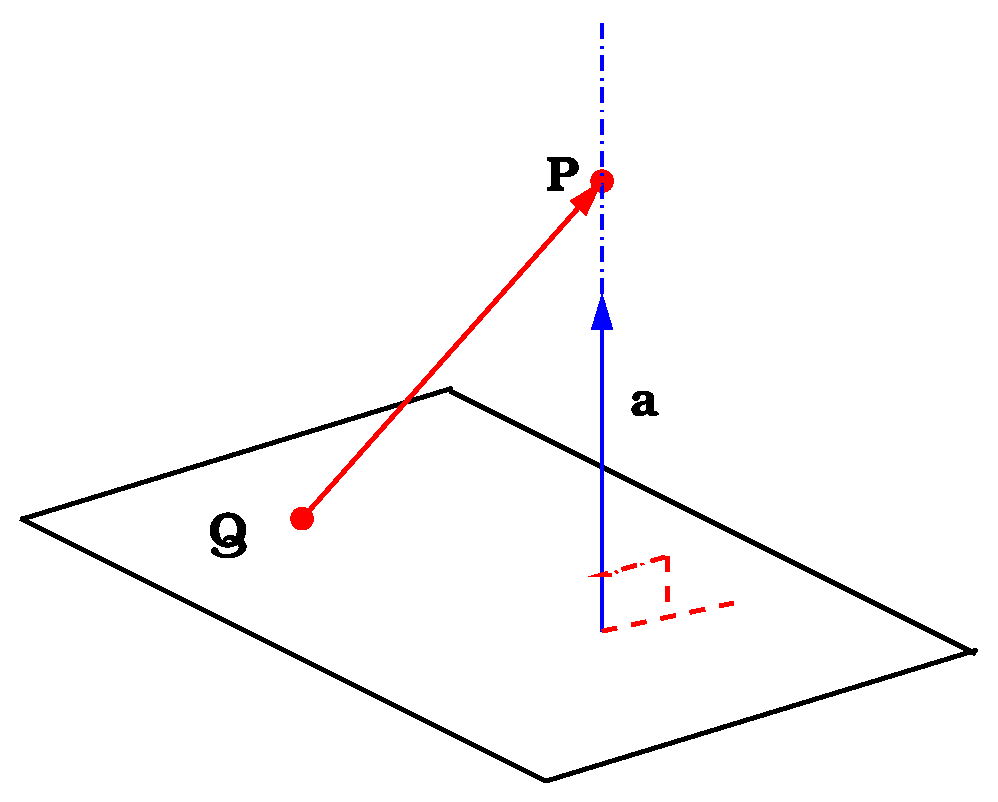
\includegraphics[width=0.6\textwidth]{xfig_stuff/distance_point_plane.fi.eps}
  \caption{$|porj_{a}(P-Q)| $ is the distance from $P$ to the plane.}
  \label{fig:distance_point_plane}
\end{figure}
The angle between plane (~\ref{eq:a_n_hyperplane_1}) and
$$
c_1 \cdot x_1 \; + \; c_2 \cdot x_2 \; + \;\dots \;+ c_n\cdot x_n \;= \; b
$$
is the angle $\hat{ac}$ between $a = (a_1,\;a_2,\; \dots\;a_n)$ and $c=(c_1,\;c_2,\;\dots\; c_n).$

\begin{center}
\begin{picture}(60,1)
\thicklines
\put(0,0){\line(1,0){60}}
\end{picture}
\end{center}
\begin{example}
  The angle between
$$
x_1+x_2+x_3+x_4 =1
$$
and
$$
x_2+x_3=1
$$
is equal to the angle between
$$
(1,\;1,\;1,\;1)\;\;\mbox{ and }\;\;(0,\;1,\;1,\;0).
$$

It follows from
$$
(1,\;1,\;1,\;1)\cdot (0,\;1,\;1,\;0)=2
$$
and
$$
|(1,\;1,\;1,\;1)|=2,\;\;|(0,\;1,\;1,\;0)|=\sqrt{2}
$$
that the angle is
$$
arccos(\frac{1}{\sqrt{2}}) =\frac{\pi}{4}.
$$
\end{example}
\begin{center}
\begin{picture}(60,1)
\thicklines
\put(0,0){\line(1,0){60}}
\end{picture}
\end{center}

\section{\href{https://en.wikipedia.org/wiki/Exterior_algebra}{Wedge product (Exterior product)}}
The \href{https://en.wikipedia.org/wiki/Exterior_algebra}{wedge product}
$$
a\wedge b
$$
of $a,\;b\in \mathbb{R}^n$ is defined by the following two properties.\\
It is antisymmetric (and/or skew-symmetric)
$$
a\wedge b = - b\wedge a
$$
and it is \href{https://en.wikipedia.org/wiki/Bilinear_map}{bilinear}, you can open parenthesis and factor out numbers
$$
(\alpha \cdot a + \beta \cdot c) \wedge b = \alpha \cdot a\wedge b + \beta \cdot c\wedge b
$$
where $\alpha,\; \beta$ are numbers and $a,\;b,\;c \in \mathbb{R}^n.$ \\
Let $\{e_1,\;e_2,\;\dots\;e_n\}$ be the canonical basis in $\mathbb{R}^n$ (see section ~\ref{sec:nspace}). Then
\begin{eqnarray*}
a&=&a_1 \cdot e_1 + a_2 \cdot e_2 + \dots + a_n \cdot e_n\\
b&=&b_1 \cdot e_1 + b_2 \cdot e_2 + \dots + b_n \cdot e_n
\end{eqnarray*}
and
$$
a\wedge b = \sum_{i<j} (a_i \cdot b_j - a_j \cdot b_i) \cdot  e_i \wedge e_j
$$
where $i,\; j$ are taking values  $1,\;2,\;\dots\; n.$\\

Let \href{https://en.wikipedia.org/wiki/Binomial_coefficient}{$\displaystyle{ n \choose 2}$}  denote the number of ways one can choose an unordered pair of elements from the set of $n$ elements. \href{https://en.wikipedia.org/wiki/Binomial_coefficient}{$\displaystyle{ n \choose 2}$} is called \href{https://en.wikipedia.org/wiki/Binomial_coefficient}{a binomial coefficient} and
$$
\displaystyle{ n \choose 2} = \frac{n!}{2! \cdot (n-2)!}
$$
where $n!= 1\cdot 2\cdot \dots \cdot n,$ the product of all natural numbers from $1$ to $n.$\\

Then
$$
a \wedge b = \sum_{i<j} \det\left( \begin{array}{cc}
                                       a_i & a_j \\
                                       b_i & b_j
                                   \end{array}\right) \cdot  e_i \wedge e_j
$$

and $a \wedge b$ is the string of values
$$
 \det\left( \begin{array}{cc}
                                       a_i & a_j \\
                                       b_i & b_j
                                   \end{array}\right) \;\;\qquad \;\; j<j\;\;\mbox{ and } i,j = 1,\;2,\;\dots \; n
$$
in $\displaystyle{ n \choose 2}$-dimensional real space with the canonical basis
$$
e_i \wedge e_j \;\;\qquad \;\; j<j\;\;\mbox{ and } i,j = 1,\;2,\;\dots \; n
$$
It is convenient to order pairs $(i,\;j)$ according to \href{https://en.wikipedia.org/wiki/Lexicographic_order}{the lexicographic rule} (like words in a dictionary).  For example, if $n=4$ then \href{https://en.wikipedia.org/wiki/Lexicographic_order}{the lexicographical order} of $(i,\;j)\;\;(i<j\;\mbox{ and }\;i,j=1,\;2,\;3,\;4)$ looks as follows.
$$
(1,\;2),\;(1,\;3),\;(1,\;4),\;(2,\;3),\;(2,\;4),\;(3,\;4)
$$
If $a,\;b \in \mathbb{R}^4$ then the wedge product $a\wedge b$ has the following coordinates.
$$
\det\left( \begin{array}{cc}
                                       a_1 & a_2 \\
                                       b_1 & b_2
                                   \end{array}\right), \det\left( \begin{array}{cc}
                                       a_1 & a_3 \\
                                       b_1 & b_3
                                   \end{array}\right), \det\left( \begin{array}{cc}
                                       a_1 & a_4 \\
                                       b_1 & b_4
                                   \end{array}\right),
$$
$$
 \det\left( \begin{array}{cc}
                                       a_2 & a_3 \\
                                       b_2 & b_3
                                   \end{array}\right), \det\left( \begin{array}{cc}
                                       a_2 & a_4 \\
                                       b_2 & b_4
                                   \end{array}\right),
$$
$$
 \det\left( \begin{array}{cc}
                                       a_3 & a_4 \\
                                       b_3 & b_4
                                   \end{array}\right)
$$
The set of all possible wedge products between strings from $\mathbb{R}^n$  is denoted by ${\bigwedge}_2 (\mathbb{R}^n),$
$$
{\bigwedge}_2 (\mathbb{R}^n) = \{a\wedge b;\; a \mbox{ and } b \in \mathbb{R}^n \}
$$

Now we consider the wedge product of several strings from $\mathbb{R}^n,$
$$
v_1\wedge v_2 \wedge \dots \wedge v_p
$$
where $ v_1,\; v_2, \; \dots \; v_p$ are from $\mathbb{R}^n$ and $ p \le  n.$ This product is linear with respect to each $v_j\;\;(j=1,\;2\;\dots \;p),$
$$
v_1\wedge v_2 \wedge \dots \wedge v_{j-1}\wedge (\alpha \cdot \bar{v_j}+\beta \cdot \hat{v_j})\wedge \dots \wedge v_p =
$$
$$
\alpha \cdot v_1\wedge v_2 \wedge \dots \wedge v_{j-1}\wedge \bar{v_j}\wedge \dots \wedge v_p + \beta \cdot  \cdot v_1\wedge v_2 \wedge \dots \wedge v_{j-1}\wedge \hat{v_j}\wedge \dots \wedge v_p
$$
where $\alpha,\; \beta \in \mathbb{R}$ and $\bar{v_j} ,\; \hat{v_j} \in \mathbb{R}^n.$\\
It is also antisymmetric (and/or skew-symmetric). It changes its sign when you flip any two $v_j,\;v_k.$
$$
v_1\wedge v_2 \wedge \dots \wedge v_{j-1}\wedge v_j\wedge \dots \wedge v_{k-1}\wedge v_k\wedge \dots \wedge v_p = - v_1\wedge v_2 \wedge \dots \wedge v_{j-1}\wedge v_k\wedge \dots \wedge v_{k-1}\wedge v_j\wedge \dots \wedge v_p
$$
Taking into account 
$$
v_j = v_{j\;1} \cdot e_1\;+\;v_{j\; 2} \cdot e_2 + \; \dots \; + v_{j\;n}\cdot e_n\;\;\;j\; =\; 1,\;2,\;\dots \; p
$$
we have 
$$
v_1\wedge v_2 \wedge \dots \dots \wedge v_p = \sum_{j_1<j_2<\dots<j_p} d(v;j_1,\;j_2,\;\dots\;j_p)\cdot e_{j_1}\wedge e_{j_2} \wedge \dots \wedge e_{j_p}
$$
where
%Let us introduce notation,
\begin{equation}
\label{eq:p_wedge_coordinates}
d(v;j_1,\;j_2,\;\dots\;j_p) = \det \left( \begin{array}{cccc}
                                         v_{1\;j_1}&v_{1\;j_2}&\dots&v_{1\;j_p}\\
                                         v_{2\;j_1}&v_{2\;j_2}&\dots&v_{2\;j_p}\\
                                          \vdots & \vdots & \vdots &\vdots \\
                                         v_{p\;j_1}&v_{p\;j_2}&\dots&v_{p\;j_p}
                                         \end{array}\right)
\end{equation}
and $j_1,\;j_2,\;\dots\;j_p$ are taking values $1,\;2,\;\dots \;n.$\\
Thus
$$
{\bigwedge}_p (\mathbb{R}^n) = \{ v_1\wedge v_2 \wedge \dots \dots \wedge v_p ;\;v_j\; \in \; \mathbb{R}^n\;(j=1\;2,\; \dots \;p)\} 
$$ 
is a subset of a $\displaystyle{ n \choose p}$-dimensional real linear space, where $\displaystyle{ n \choose p}$ denote the number of ways one can choose an unordered set of $p$ elements from the set of $n$ elements. \href{https://en.wikipedia.org/wiki/Binomial_coefficient}{$\displaystyle{ n \choose p}$} is called \href{https://en.wikipedia.org/wiki/Binomial_coefficient}{a binomial coefficient} and
$$
\displaystyle{ n \choose p} = \frac{n!}{p! \cdot (n-p)!}
$$
\begin{theorem}
The canonical basis of $\displaystyle{ n \choose p}$-dimensional real linear space is
\begin{equation}
\label{eq:wedge_canonical_basis}
\{e_{j_1}\wedge e_{j_2} \wedge \dots \wedge e_{j_p}\;;\;j_1<j_2<\dots<j_p\;\;\mbox{ and }\;\;j_k=1,\;2,\;\dots \;n,\;\mbox{ where }\;k=1,\;2,\;\dots \; p\}
\end{equation}
\end{theorem} 
\begin{proof}
We need to prove that the set (~\ref{eq:wedge_canonical_basis}) is linearly independent (see definition ~\ref{def:linear_independence} in section ~\ref{sec:nspace}). Consider
\begin{equation}
\label{eq:wedge_basis_proof}
 \sum_{j_1<j_2<\dots<j_p} \alpha_{j_1,\;j_2,\;\dots\;j_p}\cdot e_{j_1}\wedge e_{j_2} \wedge \dots \wedge e_{j_p}=0.
\end{equation}
For any 
$$
\bar j_1,\;\bar j_2,\;\dots\;\bar j_p\;\;\;(\bar j_1<\;\bar j_2<\;\dots\;< \bar j_p)
$$
 in (~\ref{eq:wedge_basis_proof}) there exists a unique ordered set
$$
k_1,\;k_2,\;\dots\;k_{n-p}  \;\;\; (k_1<\;k_2<\;\dots\;<k_{n-p} )
$$
such that after some permutations
$$
\bar j_1,\;\bar j_2,\;\dots\;\bar j_p,\; k_1,\;k_2,\;\dots\;k_{n-p}
$$ 
becomes
$$
1,\;2,\;\dots\;n
$$
Taking wedge product between the sum from (~\ref{eq:wedge_basis_proof}) and
$$
 e_{k_1}\wedge e_{k_2} \wedge \dots \wedge e_{k_{n-p}}
$$
yields
$$
(\sum_{j_1<j_2<\dots<j_p} \alpha_{j_1,\;j_2,\;\dots\;j_p}\cdot e_{j_1}\wedge e_{j_2} \wedge \dots \wedge e_{j_p})\wedge ( e_{k_1}\wedge e_{k_2} \wedge \dots \wedge e_{k_{n-p}})=0
$$
Opening the parenthesis we conclude that all terms 
$$
e_{j_1}\wedge e_{j_2} \wedge \dots \wedge e_{j_p}\wedge  e_{k_1}\wedge e_{k_2} \wedge \dots \wedge e_{k_{n-p}}
$$
in 
$$
\sum_{j_1<j_2<\dots<j_p} \alpha_{j_1,\;j_2,\;\dots\;j_p}\cdot e_{j_1}\wedge e_{j_2} \wedge \dots \wedge e_{j_p}\wedge  e_{k_1}\wedge e_{k_2} \wedge \dots \wedge e_{k_{n-p}}=0
$$
 are zeroes but one,
$$
\alpha_{\bar j_1,\;\bar j_2,\;\dots\;\bar j_p}\cdot  e_{\bar j_1}\wedge e_{\bar j_2} \wedge \dots \wedge e_{\bar j_p}\wedge  e_{k_1}\wedge e_{k_2} \wedge \dots \wedge e_{k_{n-p}}=0
$$
Hence,
$$
\alpha_{\bar j_1,\;\bar j_2,\;\dots\;\bar j_p} =0
$$
It is true for all coefficients in (~\ref{eq:wedge_basis_proof}).
Thus the set (~\ref{eq:wedge_canonical_basis}) is linearly independent. 
\vspace{0.1cm}
Q.E.D.
\vspace{0.1cm}
\end{proof} 
For $v_1,\;v_2,\;\dots\; v_p\;\in\;\mathbb{R}^n$ the wedge product $v_1\wedge \;v_2\wedge \;\dots\; \wedge v_p$
has the following coordinates
$$
\{ d(v;j_1,\;j_2,\;\dots\;j_p)\}_{j_1<j_2<\dots<j_p } 
$$
where $d(v;j_1,\;j_2,\;\dots\;j_p)$ is defined in (~\ref{eq:wedge_canonical_basis}) and $j_1,\;j_2,\;\dots\;j_p$ are lexicographically ordered.
\subsection{Wedge product in Euclidean space}
A linear real space $\mathbb{R}^n$ with the dot product 
$$
x\cdot y = x_1 \cdot y_1 + x_2 \cdot y_2 + \dots + x_n \cdot y_n
$$
is called a Euclidean space (see section ~\ref{sec:Euclidean_space}).  One can calculate all sorts of stuff  with the help of the dot product. In particular the magnitude $|x|$ of $x$ is
$$
|x| = \sqrt{x\cdot x}
$$
 ${\bigwedge}_p (\mathbb{R}^n)$ is a subset of Euclidean space as well and we can use the following dot product.
$$
(w_1\wedge \;w_2\wedge \;\dots\; \wedge w_p)\cdot (v_1\wedge \;v_2\wedge \;\dots\; \wedge v_p) = \sum_{j_1<j_2<\dots<j_p} d(w;j_1,\;j_2,\;\dots\;j_p)\cdot d(v;j_1,\;j_2,\;\dots\;j_p)
$$
The magnitude $|v_1\wedge \;v_2\wedge \;\dots\; \wedge v_p|$ is
$$
|v_1\wedge \;v_2\wedge \;\dots\; \wedge v_p| = \sqrt{ \sum_{j_1<j_2<\dots<j_p} (d(v;j_1,\;j_2,\;\dots\;j_p))^2  }
$$
There is another way to calculate $|v_1\wedge \;v_2\wedge \;\dots\; \wedge v_p|,$
\begin{equation}
\label{eq:wedge_volume}
|v_1\wedge \;v_2\wedge \;\dots\; \wedge v_p| = Vol (v_1, \;v_2, \;\dots\;  v_p)
\end{equation}
where $Vol$ is from (~\ref{mvolume}) (see definition ~\ref{def:mvolume}) . We prove (~\ref{eq:wedge_volume}) only for $p=2.$ It will illustrate the main idea behind (~\ref{eq:wedge_volume}). \\

   Consider $a,\; b\in \mathbb{R}^n.$ $a\wedge b$ is the list of determinants
$$
\left\{ \det\left( \begin{array}{cc}
                                       a_i & a_j \\
                                       b_i & b_j
                                   \end{array}\right)\right\}_{i<j}
$$
where $i,j=1,\;2,\;\dots \;n.$ Therefore
$$
|a\wedge b|^2 =  \sum_{i < j} \det\left( \begin{array}{cc}
                                       a_i & a_j \\
                                       b_i & b_j
                                   \end{array}\right)^2
$$
We need to prove that 
$$
 \det\left( \begin{array}{cc}
                                       a\cdot a & a\cdot b \\
                                       b\cdot a & b \cdot b
                                   \end{array}\right) =  \sum_{i < j} \det\left( \begin{array}{cc}
                                       a_i & a_j \\
                                       b_i & b_j
                                   \end{array}\right)^2
$$
It follows from
$$
\left( \begin{array}{c}
          a\cdot a\\
          b\cdot a
       \end{array} \right) =\sum_{i=1}^n a_i \cdot \left( \begin{array}{c}
                                                                a_i\\
                                                                b_i
                                                           \end{array} \right)
$$
and, respectively,
$$
\left( \begin{array}{c}
          a\cdot b\\
          b\cdot b
       \end{array} \right) =\sum_{i=1}^n b_i \cdot \left( \begin{array}{c}
                                                                a_i\\
                                                                b_i
                                                           \end{array} \right)
$$
that
$$
\det\left( \begin{array}{cc}
                                       a\cdot a & a\cdot b \\
                                       b\cdot a & b \cdot b
                                   \end{array}\right) =
 \det\left( \begin{array}{cc}
 \left( \begin{array}{c}
          a\cdot a\\
          b\cdot a
       \end{array} \right)  &
\left( \begin{array}{c}
          a\cdot b\\
          b\cdot b
       \end{array} \right)
                                   \end{array}\right) =
$$
$$
 \det\left( \begin{array}{cc}
\sum_{i=1}^n a_i \cdot
 \left( \begin{array}{c}
                a_i\\
                b_i
     \end{array} \right) &
\left( \begin{array}{c}
          a\cdot b\\
          b\cdot b
       \end{array} \right)
                                   \end{array}\right) = \sum_{i=1}^n a_i \cdot  \det\left( \begin{array}{cc}
 \left( \begin{array}{c}
                a_i\\
                b_i
     \end{array} \right) &
\left( \begin{array}{c}
          a\cdot b\\
          b\cdot b
       \end{array} \right)
                                   \end{array}\right)
$$
Performing the same steps for
$$
\left( \begin{array}{c}
          a\cdot b\\
          b\cdot b
       \end{array} \right)
$$
yields
$$
\det\left( \begin{array}{cc}
 \left( \begin{array}{c}
          a\cdot a\\
          b\cdot a
       \end{array} \right)  &
\left( \begin{array}{c}
          a\cdot b\\
          b\cdot b
       \end{array} \right)
                                   \end{array}\right) = \sum_{i,j=1}^n a_i b_j
 \det\left( \begin{array}{cc}
                                       a_i & a_j \\
                                       b_i & b_j
                                   \end{array}\right)
$$
Taking into account properties of the determinant
$$
 \det\left( \begin{array}{cc}
                                       a_i & a_j \\
                                       b_i & b_j
                                   \end{array}\right) = - \det\left( \begin{array}{cc}
                                       a_j & a_i \\
                                       b_j & b_i
                                   \end{array}\right)
$$
we obtain
$$
\det\left( \begin{array}{cc}
                                       a\cdot a & a\cdot b \\
                                       b\cdot a & b \cdot b
                                   \end{array}\right)=
\sum_{i<j} (a_i b_j - a_j b_i)
 \det\left( \begin{array}{cc}
                                       a_i & a_j \\
                                       b_i & b_j
                                   \end{array}\right)
$$
and finally
$$
\det\left( \begin{array}{cc}
                                       a\cdot a & a\cdot b \\
                                       b\cdot a & b \cdot b
                                   \end{array}\right)=
\sum_{i<j}
 \det\left( \begin{array}{cc}
                                       a_i & a_j \\
                                       b_i & b_j
                                   \end{array}\right)^2
$$

\subsection{Star operator $\ast $ }
Consider the wedge product
$$
v_1\wedge v_2 \wedge \dots \wedge v_p
$$
where $ v_1,\; v_2, \; \dots \; v_p$ are from $\mathbb{R}^n$
 and $ p \le  n.$ The set of all such wedge products is denoted by
$$
{\bigwedge}_p(\mathbb{R}^n)
$$
It is a subset of a linear space of dimension ${n \choose p}.$\\
Let
$$
v_1\wedge v_2 \wedge \dots \wedge v_p = \sum_{i_1 < i_2<\dots <i_p} x_{i_1 i_2 \dots \i_p} e_{i_1}\wedge e_{i_2} \wedge \dots \wedge e_{i_p}
$$
Then the star operator
$$
\ast : \; {\bigwedge}_p(\mathbb{R}^n) \to {\bigwedge}_{n-p}(\mathbb{R}^n)
$$
is a linear mapping defined as follows.
$$
\ast(v_1\wedge v_2 \wedge \dots \wedge v_p) = \sum_{i_1 < i_2<\dots <i_p} x_{i_1 i_2 \dots \i_p}(\ast( e_{i_1}\wedge e_{i_2} \wedge \dots \wedge e_{i_p}))
$$
where
$$
\ast( e_{i_1}\wedge e_{i_2} \wedge \dots \wedge e_{i_p}) = (-1)^{P(j_1,\; \dots \; j_{n-p}, \; i_1 \; \dots \; i_p)}  e_{j_1}\wedge e_{j_2} \wedge \dots \wedge e_{j_{n-p}}
$$
and $j_1 < j_2<\dots <j_{n-p}$  is such that one can get
$$
(1,\;2,\;\dots \; n)
$$
out of
$$
 j_1,\; \dots \; j_{n-p}, \; i_1 \; \dots \; i_p
$$
performing the number $P(j_1,\; \dots \; j_{n-p}, \; i_1 \; \dots \; i_p)$ of \href{https://en.wikipedia.org/wiki/Cyclic_permutation#Transpositions}{transpositions.}

\vspace{0.1cm}

For example ${\bigwedge}_2 (\mathbb{R}^3)$ has the following canonical basis.
$$
e_1 \wedge e_2,\;e_1 \wedge e_3,\; e_2\wedge e_3
$$
One makes $(1,\;2,\;3)$ out of $(3,\;1,\;2)$ with $2$ \href{https://en.wikipedia.org/wiki/Cyclic_permutation#Transpositions}{transpositions} and
$$
\ast(e_1 \wedge e_2) = (-1)^2 e_3 = e_3
$$
After flipping $2$ and $1$ (one transposition) $(2,\;1,\;3)$ becomes $(1,\;2,\;3) $ and
$$
\ast(e_1 \wedge e_3) = (-1)^1 e_2 = -e2
$$
Finally
$$
\ast(e_2 \wedge e_3) = (-1)^0 e_1 = e_1
$$
For any $a,\;b \in \mathbb{R}^3$
$$
a\wedge b =  \det\left( \begin{array}{cc}
                                       a_1 & a_2 \\
                                       b_1 & b_2
                                   \end{array}\right) e_1\wedge e_2 +
             \det\left( \begin{array}{cc}
                                       a_1 & a_3 \\
                                       b_1 & b_3
                                   \end{array}\right) e_1 \wedge e_3 +
             \det\left( \begin{array}{cc}
                                       a_2 & a_3 \\
                                       b_2 & b_3
                                   \end{array}\right) e_2 \wedge e_3
$$
and
$$
\ast(a \wedge b) = \det\left( \begin{array}{cc}
                                       a_1 & a_2 \\
                                       b_1 & b_2
                                   \end{array}\right)(\ast ( e_1\wedge e_2)) +
             \det\left( \begin{array}{cc}
                                       a_1 & a_3 \\
                                       b_1 & b_3
                                   \end{array}\right)(\ast ( e_1 \wedge e_3)) +
             \det\left( \begin{array}{cc}
                                       a_2 & a_3 \\
                                       b_2 & b_3
                                   \end{array}\right)(\ast (e_2 \wedge e_3))
$$
Taking into account $\ast(e_1\wedge e_2)=e_3,\;\;\ast(( e_1 \wedge e_3)=-e2,\;\;\ast (e_2 \wedge e_3)=e1$ yields the following.
$$
\ast(a \wedge b)=\det\left( \begin{array}{cc}
                                       a_1 & a_2 \\
                                       b_1 & b_2
                                   \end{array}\right) e_3 +
             \det\left( \begin{array}{cc}
                                       a_1 & a_3 \\
                                       b_1 & b_3
                                   \end{array}\right)(-e_2) +
             \det\left( \begin{array}{cc}
                                       a_2 & a_3 \\
                                       b_2 & b_3
                                   \end{array}\right) e_1
$$
You can see that $\ast(a \wedge b)$ is identified by the following string from  $\mathbb{R}^3.$
$$
\left( \det\left( \begin{array}{cc}
                                       a_2 & a_3 \\
                                       b_2 & b_3
                                   \end{array}\right) , - \det\left( \begin{array}{cc}
                                       a_1 & a_3 \\
                                       b_1 & b_3
                                   \end{array}\right),
                                   \det\left( \begin{array}{cc}
                                       a_1 & a_2 \\
                                       b_1 & b_2
                                   \end{array}\right)\right)
$$
This string from $\mathbb{R}^3$ has a special name it is called the cross product between $a$ and $b$ and denoted by $a \times b .$
The cross product is defined \textcolor{red}{ONLY IN $\mathbb{R}^3$} and
$$
a \times  b = \ast (a \wedge b)\;\;\mbox{ for } a,\; b\in \mathbb{R}^3
$$
 However, 
$$
 \ast (a \wedge b)\;\;\mbox{ where } a,\; b \in \mathbb{R}^n
$$
is valid for any $n.$ In particular for $n=4$, in time-space continuum,  $\ast (a \wedge b)$ has six entries. Three of them coincide with the spatial cross product and the other three involve time. Indeed, if $a,\; b\in \mathbb{R}^4$ then
\begin{eqnarray*}
a\wedge b &= & \det\left( \begin{array}{cc}
                                       a_1 & a_2 \\
                                       b_1 & b_2
                                   \end{array}\right) e_1\wedge e_2 +
             \det\left( \begin{array}{cc}
                                       a_1 & a_3 \\
                                       b_1 & b_3
                                   \end{array}\right) e_1 \wedge e_3 +
             \det\left( \begin{array}{cc}
                                       a_1 & a_4 \\
                                       b_1 & b_4
                                   \end{array}\right) e_1 \wedge e_4 +\\
 & & \det\left( \begin{array}{cc}
                                       a_2 & a_3 \\
                                       b_2 & b_3
                                   \end{array}\right) e_2\wedge e_3 +
             \det\left( \begin{array}{cc}
                                       a_2 & a_4 \\
                                       b_2 & b_4
                                   \end{array}\right) e_2 \wedge e_4 +
             \det\left( \begin{array}{cc}
                                       a_3 & a_4 \\
                                       b_3 & b_4
                                   \end{array}\right) e_3 \wedge e_4 
\end{eqnarray*}
and
\begin{eqnarray*}
\ast(a\wedge b) &= & \det\left( \begin{array}{cc}
                                       a_1 & a_2 \\
                                       b_1 & b_2
                                   \end{array}\right) \ast (e_1\wedge e_2) +
             \det\left( \begin{array}{cc}
                                       a_1 & a_3 \\
                                       b_1 & b_3
                                   \end{array}\right) \ast(e_1 \wedge e_3) +
             \det\left( \begin{array}{cc}
                                       a_1 & a_4 \\
                                       b_1 & b_4
                                   \end{array}\right) \ast (e_1 \wedge e_4) +\\
 & & \det\left( \begin{array}{cc}
                                       a_2 & a_3 \\
                                       b_2 & b_3
                                   \end{array}\right) \ast(e_2\wedge e_3) +
             \det\left( \begin{array}{cc}
                                       a_2 & a_4 \\
                                       b_2 & b_4
                                   \end{array}\right) \ast(e_2 \wedge e_4) +
             \det\left( \begin{array}{cc}
                                       a_3 & a_4 \\
                                       b_3 & b_4
                                   \end{array}\right) \ast(e_3 \wedge e_4 )
\end{eqnarray*}
It follows from 
\begin{eqnarray*}
\ast (e_1\wedge e_2) &=& e_3 \wedge e_4\\
\ast (e_1\wedge e_3) &=& -e_2 \wedge e_4\\
\ast (e_1\wedge e_4) &=& e_2 \wedge e_3\\
\ast (e_2\wedge e_3) &=& e_1 \wedge e_4\\
\ast (e_2\wedge e_4) &=& -e_1 \wedge e_3\\
\ast (e_3\wedge e_4) &=& e_1 \wedge e_2\\
\end{eqnarray*}
that
\begin{eqnarray*}
\ast(a\wedge b) &= & \det\left( \begin{array}{cc}
                                       a_3 & a_4 \\
                                       b_3 & b_4
                                   \end{array}\right) e_1\wedge e_2 -
             \det\left( \begin{array}{cc}
                                       a_2 & a_4 \\
                                       b_2 & b_4
                                   \end{array}\right) e_1 \wedge e_3 +
             \det\left( \begin{array}{cc}
                                       a_2 & a_3 \\
                                       b_2 & b_3
                                   \end{array}\right) e_1 \wedge e_4 +\\
 & & \det\left( \begin{array}{cc}
                                       a_1 & a_4 \\
                                       b_1 & b_4
                                   \end{array}\right) e_2\wedge e_3 -
             \det\left( \begin{array}{cc}
                                       a_1 & a_3 \\
                                       b_1 & b_3
                                   \end{array}\right) e_2 \wedge e_4 +
             \det\left( \begin{array}{cc}
                                       a_1 & a_2 \\
                                       b_1 & b_2
                                   \end{array}\right) e_3 \wedge e_4 
\end{eqnarray*}
Hence, $\ast(a\wedge b) $ is represented by the following string from $\mathbb{R}^6.$
$$
\left(
\textcolor{blue}{
\det\left( \begin{array}{cc}
                a_3 & a_4 \\
                b_3 & b_4
       \end{array}\right),\;
       -\det\left( \begin{array}{cc} 
                a_2 & a_4 \\            
                b_2 & b_4
                   \end{array}\right),\;
}
\textcolor{red}{
       \det\left( \begin{array}{cc}
                a_2 & a_3 \\
                b_2 & b_3
                  \end{array}\right),\;
}
\right.
$$
$$
\left. 
\textcolor{blue}{
      \det\left( \begin{array}{cc}
                a_1 & a_4 \\
                b_1 & b_4
                   \end{array}\right),\;
}
\textcolor{red}{
       -\det\left( \begin{array}{cc}
                 a_1 & a_3 \\
                 b_1 & b_3
                   \end{array}\right),\;
        \det\left( \begin{array}{cc}
                a_1 & a_2 \\
                b_1 & b_2
                   \end{array}\right)
}
 \right)
$$
If we treat $x_1,\;x_2,\;x_3$ as spatial variables ($x,\;y,\;z$ in common textbooks) and $x_4$ as time (it is usually marked by $t)$ then three entries in the low right corner (typed in red ) correspond to \href{https://en.wikipedia.org/wiki/Cross_product}{the traditional spatial cross product}  and three entries in the upper left corner (those in blue) are not in wide use by humans yet. They are related to time and space.

\section{One-to-one mapping of $(0,\;1)\times (0,\;1)$ to $(0,\;1)$}
The goal of this section is to describe a one-to-one mapping of the unit square into the unit interval. The square is $(0,\; 1)\times (0,\;1)$ which means
$$
(0,\; 1)\times (0,\;1) =\{ (x_1,\;x_2); \mbox{ where } x_1 \mbox{ and } x_2 \mbox{ are from } (0,\;1)\} 
$$
Let us take a point from $(0,\; 1)\times (0,\;1)$
$$
(x_1,\;x_2) = (0.a_1a_2a_3\dots,\;0.b_1b_2b_3\dots)
$$
We may need to append zeroes either to $0.a_1a_2a_3\dots$ or to $0.b_1b_2b_3\dots$ in order to have them of the same length. Then we can do the process called mixing.
$$
(0.a_1a_2a_3\dots,\;0.b_1b_2b_3\dots) \;\; \rightarrow \;\; 0.a_1b_1a_2b_2a_3b_3\dots
$$
This mapping is one-to-one if you prohibit rounding up and treat $0.1$ and $0.0999\dots 9\dots$ as different numbers. However, according the current state of mathematical knowledge
$$
0.1 = 0.0999\dots 9\dots
$$
It is the same in all similar situations. It breaks our mixing in the following way.\\
For example,
$$
(0.1, 0.25) = (0.10,0.25) \;\; \rightarrow   0.1205
$$
at the same time (at the current state of knowledge on the planet earth)
$$
(0.1, 0.25) \ = (0.0999...9{\dots}, 0.25000...0{\dots})\;\; \rightarrow \;\; 0.0295909090\dots 90\dots
$$
as you can see $ 0.1205 \neq 0.0295909090{\dots} 90{\dots}.$\\
In order to fix this problem we do the following.
$$
 (0,\;1) \times (0,\;1)  \;\;\rightarrow \;\; \mbox{ rounding up }  \;\;\rightarrow \;\;  \mbox{ mixing } \;\;\rightarrow \;\; (0,\;1)
$$
Going back to the example of mapping
$$
(0.1, 0.25)  \;\;\rightarrow \;\; 0.1205
$$
we see that 
$$
(0.0999{\dots}9{\dots}, 0.25000{\dots}0{\dots}) \;\;\rightarrow \;\; \mbox{ rounding up }  \;\;\rightarrow \;\; (0.1, 0.25) \;\;\rightarrow \;\;  \mbox{ mixing } \;\;\rightarrow \;\; 0.1205
$$
Our mapping
\begin{figure}[htbp]
  \centering
  \includegraphics[width=0.6\textwidth]{image/Round_up_mixing.png}
  \caption{Correctly defined injection of $(0,\;1)\times (0,\;1)$ into  $(0,\;1)$}
  \label{fig:distance_point_plane}
\end{figure}
is correctly defined now. It is injection of $(0,\;1)\times (0,\;1)$ into  $(0,\;1).$ Its image does not cover all interval $(0,\;1)$ because of rounding up. We excluded the results of mixing those points $(x_1,\;x_2)$ where either $x_1$ or $x_2$ has the tail of nines.\\

For example,
$$
(0.0999{\dots}9{\dots}, 0.25000{\dots}0{\dots})\;\; \rightarrow \;\; 0.0295909090{\dots}90{\dots}
$$
and $ 0.0295909090{\dots}90{\dots}$ does not belong to the image of our mapping.\\
In order to fix this problem we tweak our mapping (the ground for our tweaking process is provided by \href{https://en.wikipedia.org/wiki/Schr%C3%B6der%E2%80%93Bernstein_theorem}{Schr\"oder-Bernstein theorem}). In our layman terms it sounds like "kicking can down the road and staying happy ever after". In real live it can lead to catastrophic consequences but in mathematics it is OK.\\
We will tweak our mapping on the vertical segment $\{(0.5,\;y_2);\;\;y_2 \in (0,\;1)\}$ (the vertical segment can be replaced by any segment or curve inside of $ (0,\;1)\times (0,\;1)).$ The numbers from $(0,\;1)$ that have tails 
$$
9x_19x_29x_39{\dots}9x_n\dots\;\;(x_j \mbox{ is any symbol from Arabic numerals }0,\;1,\;2,\;3,\;4,\;5,\;6,\;7,\;8,\;9)
$$
are not in the image of our mapping.  Let us take such number $\alpha_0 .$ We tweak our mapping at the point $(0.5,\;\alpha_0) $ as follows. Instead of rounding and then mixing we simply project it onto $(0,\;1)$ as follows 
$$
(0.5,\; \alpha_0) \;\;\rightarrow \;\; \alpha_0
$$
We do the projection for all points $(0.5, y_{2})$ where $y_{2 }$ has the exotic tail like
\begin{equation}
\label{fancy_tail1}
 9x_{1}9x_{2}9x_{3}9{\dots}9x_{n}{\dots}
\end{equation}
where $x_j $ is any symbol from Arabic numerals $0,\;1,\;2,\;3,\;4,\;5,\;6,\;7,\;8,\;9.$\\
After that all numbers with the tails like (~\ref{fancy_tail1}) are in the image of our mapping.\\
However, by replacing mixing with projection we generated a new set of numbers that are not in the image. Those numbers are obtained by mixing points like $(0.5,\;\alpha_{0}).$ Clearly we need to look only at the tail after mixing,
\begin{eqnarray*}
000{\dots}0{\dots}&&\\
 &\rightarrow &  090x_{1}090x_{2}090{\dots}x_{n}090{\dots}\\
 9x_{1}9x_{2}9x_{3}9{\dots}9x_{n}{\dots} &&
\end{eqnarray*}
Now our image does not contain numbers $\alpha_{1}$ with the tail
$$
090x_{1}090x_{2}090{\dots}x_{n}090{\dots}
$$
where  $x_j $ is any symbol from Arabic numerals $0,\;1,\;2,\;3,\;4,\;5,\;6,\;7,\;8,\;9.$\\
For those numbers we tweak our mapping again at $(0.5,\;\alpha_{1})$ and replace mixing with the projection
$$
(0.5,\;\alpha_{1}) \;\; \rightarrow \;\; \alpha_{1}
$$
Now we do not cover numbers $\alpha_{3}$  from $(0,\;1)$ with the tail obtained by mixing
\begin{eqnarray*}
0000000000{\dots}0{\dots}&&\\
 &\rightarrow &  09000x_{1}0009000x_{2}0009000{\dots}x_{n}0009000{\dots}\\
 090x_{1}090x_{2}090x_{3}090{\dots}090x_{n}{\dots} &&
\end{eqnarray*}
We tweak our mapping again at $ (0.5,\;\alpha_{3})$ by replacing mixing with projection
$$
(0.5,\;\alpha_{3}) \;\; \rightarrow \;\; \alpha_{3}
$$
Now we can see the pattern of tweaking our mapping. Let $\alpha_{2m+1}$denote the number from $(0,\;1)$ with the tail that has $2m+1$ zeroes before and after $9,$
$$
{\dots}0{\dots}0009000{\dots}0x_{1}000{\dots}09000{\dots}0x_{2}000{\dots}09000{\dots}0{\dots}x_{n}000{\dots}09000{\dots}0{\dots}
$$
For all odd numbers $2m+1$ we tweak our mapping at $(0.5,\;\alpha_{2m+1})$ by replacing mixing with projection
$$
(0.5,\;\alpha_{2m+1}) \;\;\rightarrow \;\; \alpha_{2m+1}
$$
After tweaking our mapping on the vertical interval
$$
 \{(0.5,\; y_{2}); y_{2} \in (0,\;1)\}
$$
as described we finally obtain a one-to-one mapping of $ (0,\;1)\times (0,\;1) \;\;\rightarrow \; (0,\;1).$\\
In the same manner one constructs a one-to-one mapping of the \href{https://en.wikipedia.org/wiki/Hypercube}{hypercube} 
$$
(0,\;1)^n \;\;\rightarrow (0,\;1),
$$ 
where $(0,\;1)^2$ denotes $(0,\;1)\times (0,\;1),$  $(0,\;1)^3$ is for $(0,\;1)\times (0,\;1)\times (0,\;1)$ etc.




%%%%%%%%%%%%%%%%%%%done with conclusion

%\section{\href{https://en.wikipedia.org/wiki/Minkowski_space}{Minkowski space}}
%SergeY
%\printindex
\end{document}
